\documentclass[hidelinks,12pt,letterpaper,twoside]{book}
\usepackage[utf8]{inputenc}
\usepackage{fancyhdr}
\usepackage{hyperref}
\usepackage{geometry}
\usepackage{titletoc}% http://ctan.org/pkg/titletoc
\usepackage{afterpage}
\usepackage{tocloft}
\usepackage{multirow}
\usepackage{graphicx}
\usepackage{booktabs}
\usepackage{wrapfig}
\usepackage{amsmath}

\graphicspath{ {./images/} }

\renewcommand{\arraystretch}{1.5}

\setlength{\headheight}{110pt}

\makeatletter
\@addtoreset{chapter}{part}
\makeatother  

\newcommand\blankpage{%
    \null
    \thispagestyle{empty}%
    %\addtocounter{page}{-1}%
    \newpage}

\author{WSU Physics \& Astronomy}
\title{2131 Lab Manual}

\geometry{margin=1in}

\pagestyle{fancy}
\fancyhf{}
\fancyhead[LE,RO]{Physics 2131 Lab Manual}
\fancyhead[RE,LO]{Lab \thechapter}
\fancyfoot[LE,RO]{\thepage}

\tocloftpagestyle{fancy}

\begin{document}

\begin{titlepage}
	\centering
	
\includegraphics[width=0.15\textwidth]{wsu_logo}\par\vspace{1cm}
	{\scshape\LARGE Physics 2131 \par}
	\vspace{0.5cm}
	{\scshape\large Physics for the Life Sciences\par}
	\vfill
	\textbf{\huge Lab Manual} \par
	\vfill
% Bottom of the page
	{\scshape\large Winter 2017 \par}
	{\scshape\large \today \par}
\end{titlepage}

\newpage{\blankpage}

\clearpage
\setcounter{page}{1}

\chapter*{Physics 2131 - Syllabus}
\thispagestyle{fancy}
\fancyhead[RE,LO]{Syllabus}
The General Physics Laboratory is designed as introduction to research methods.
It focuses on applications of physics relevant to the life sciences.
Students learn how to design experiments to answer physical question, learn how to summarize and present their methods, findings and conclusions, and how to present their conclusions both in written and oral form.
Students also learn how to discuss their findings and be able to defend their conclusions.

\section*{Instructor}
Instructor: $\rule{10cm}{0.15mm}$ \\
\medskip \\ 
Email: $\rule{10cm}{0.15mm}$ \\
\medskip \\
Office: $\rule{10cm}{0.15mm}$ \\
\medskip \\
Office hours: $\rule{10cm}{0.15mm}$

\section*{Learning Outcomes}
By completing this lab course, students will be able to
\begin{itemize}
\item Design experiments, and measure \& analyze data to answer physical questions in the life sciences and related areas.
\item Use modern experimental equipment and computer analysis to measure various physical phenomena.
\item Present and discuss methods, findings and interpretation of data both in written and oral form.
\item Collaborate on a research project in a team.
\end{itemize}

\newpage

\section*{How to be successful in this course}
The key to being successful in this course is to focus on teamwork.
By working together to efficiently gather and analyze the data, your team will be free to spend more time discussing your results.
This is the true focus of this lab class: using your data to draw appropriate conclusions about the phenomena that you are investigating.
%So how can you make the best use of your time to get a good grade in this class?
\begin{itemize}
	\setlength\itemsep{2pt}
	\item \textbf{Before you come to lab:} Read over the entire lab.
	Spend some time thinking about what is involved and how you might do the experiment.
	Read through any relevant sections in the textbook even if the lecture class hasn't reached them yet.
	Communicate with your lab team to begin planning out the way you will carry out the experiment.
	\item \textbf{While you are in the lab:} Focus on your goals and tasks in the lab, don't waste time.
	If you take a lot of time on irrelevancies, you may have trouble finishing.
	Remember to document what you are doing in a lab report created as you go.
	\item \textbf{Before you leave the lab:} Be sure each team member has a copy of the data.
	You don't want to arrive in the second (or third) week and find the only person with your data has dropped the course (or is sick, or is away at a sports event, or forgot it, or ...).
	At the end of a one-week lab or the last week of a multi-week lab, hand in your finished lab report before you leave.
\end{itemize}

\section*{Roles}
In order to facilitate the preparation of the lab report, you will be working in groups of two or three.  There are three roles that your group members will fill; while each member takes primary responsibility for one role and for the portion of the lab report related to that role, please keep in mind that the experiment is a group effort and you should all be aware of the dilemmas faced by your peers and the decisions that they make.  Also, except when writing the report, these lab experiments often involve ``all hands on deck'' -- with every group member contributing to the construction, execution, and analysis of an experimental protocol.  The division of labor will be as follows:
\begin{list}{}{\itemsep=1pt} %\topsep=2pt
\item \textbf{The Journalist:} This person is primarily responsible for taking notes of everything that happens during the experiment and writing up the ``Introduction'' section of the lab report.
 
\item \textbf{The Data Interpreter:} This person primarily deals with tabulating and displaying the data, operating the computer, and writing up the ``Graphs \& Analysis'' section of the lab report. While all members of the group are expected to be involved in the collection and analysis of the results, this person is responsible for making them presentable.
 
\item \textbf{The Checker:} This person is responsible for making sure that the group is properly following the experiment plan, and makes sure that all requirements from the lab manual are being met. They are in charge of writing the ``Conclusion'' section. This person also acts as a ``manager'' of the lab tasks, stepping in where help is needed and coordinating the group's efforts to ensure the lab is completed efficiently and on-time.
\end{list}

\newpage

\section*{Grading}
\begin{itemize}
\item \textbf{ Leading a discussion:} Every student will lead a discussion 1-2 times per semester. The student will introduce a question, problem or idea, and lead a short discussion about it. Total time 5-7 minutes – \textbf{10\%} of grade (Individual)
\item \textbf{Quizzes (in-class):} Every two weeks, about previous lab, at beginning of class (15 minutes, 3-4 questions). Content: Lab techniques, units, meaning of results, etc. - \textbf{20\%} of grade (Individual)
\item \textbf{Lab reports}(see below): For the final approx.\ 30 minutes of the last day of an experiment, your lab team will work on completing a write-up of the experiment that you performed following the format listed below. - \textbf{40\%} of grade (Group)
\item \textbf{Final presentations:} Give complete overview of one of the experiments, with methods, data, discussion, questions, ideas, conclusions – 10 minutes each group - \textbf{30\%} of grade (Group)
\end{itemize}

\section*{Grading of Lab Reports}
%The lab grade makes up part of your total course grade.
%This grade will be based on your team's lab reports and your individual participation in the lab and the class discussions.
%\emph{Your grade will not depend on whether or not your numerical results agree with some accepted standard but on how well you conceived and carried out the experiment.} \\
%
\begin{tabular}{|p{13cm}|c|}
\hline
\textbf{Team Lab Report} & \textbf{Weight} \\
\hline
\emph{Design and thoughtfulness:} Did your team do a careful and thoughtful job in creating your experiment, and was this thought reflected in the journal? & 25\% \\
\hline
\emph{Clarity and completeness:} Did your team explain your experiment so that someone could reproduce it? & 25\% \\
\hline
\emph{Persuasiveness:} What conclusions did your team draw from your data and were you able to back up these conclusions with this data in a convincing way? & 25\% \\
\hline
\emph{Evaluation:} After observing the experiments of other groups, were you able to critique your own lab, propose constructive changes, or explain why your experiment was better than those of your classmates?  (The question you are answering in your evaluation is, ``If I got to re-do this experiment next week, how would I do it differently?'') & 25\% \\
\hline
%\textbf{Individual Participation} & \\
%\hline
%\emph{Contribution to team presentation:} Did you participate constructively in your own group's work (protocol development and data collection)?  Did you actively participate in both the preparation of the report/presentation and its delivery? & 10\% \\
%\hline
%\emph{Contribution of other teams' presentations:} Did you ask useful questions or make comments that were valuable to the other teams' reports of their evaluations?  Did you participate in both class and small group discussion? & 10\% \\
%\hline
\end{tabular}
%
%\bigskip 
%More specific rubrics may be provided for each lab report [e.g., with directions for graphs to include], but the guidelines provided in the table above will be used to evaluate all lab reports.

\newpage

\section*{Lab Reports}
Each group will work together to submit one lab report for each experiment they complete.
The lab report must be submitted electronically to your lab TA at the end of each experiment, late submissions will not be accepted unless under extenuating circumstances.

\subsection*{Introduction \& Methods}
This section should begin with a description of the process you are investigating.
Describe what data you plan to gather and explain how it will be useful in your investigation.
Briefly describe the steps you took to gather that data and the methods you used to analyze your results. \\
\textbf{Requirements}
\begin{list}{-}{\topsep=0pt \itemsep=0pt}
	\item At least one paragraph in length
	\item Simple figures may be used to illustrate the experimental setup
	\item Explain any equations that you will be using in the course of your data analysis
	\item Be detailed but avoid minutia! No one needs to read the full details of every single step you took. 
\end{list}

\subsection*{Graphs \& Analysis}
This section should include graphs of the data that you mentioned in the introduction.
The lab manual will guide you on the number of graphs that you should aim to include, but feel free to add more if you feel they are relevant.
After each graph, include a few sentences explaining it: point out important features, comment on the fit of the data against any theoretical curves, etc. \\
\textbf{Requirements}
\begin{list}{-}{\topsep=0pt \itemsep=0pt}
	\item All axes must be well labeled at a legible size and with appropriate units
	\item Use reasonable significant figures
	\item Calculate uncertainty whenever possible and use error bars.
	\item Don't skimp out on the explanations after each graph, as this is probably the most critical part of any report. Don't rely on the reader to make the connection between what is in the graph and the phenomena you are investigating, tell them explicitly.
\end{list}

\subsection*{Conclusion}
In this section you want to demonstrate how all your results connect to elucidate the phenomena you set out to investigate.
Discuss the strongest and weakest areas of your investigation, and describe changes that you would make to your experimental plan if you were to repeat your work.
If possible, discuss how the things that you learned about in each experiment would be applicable to topics studied in other science classes.

\section*{Schedule}
Below is a preliminary schedule for the Winter 2017 semester.
This schedule is subject to change due to unforeseen circumstances, any changes will be announced via blackboard. \\

\begin{tabular}{ |c|c|l|c| } 
 \hline
 \textbf{Week} & \textbf{Week Begins} & \textbf{Content}  & \textbf{Quiz} \\ 
 \hline
    & Jan. 9 & \textbf{No Class} & \\ 
 \hline 
%  1 & Jan. 9 & Introduction \& Equipment walkthrough \\ 
% \hline 
    & Jan. 16 & \textbf{No Class} & \\ 
 \hline
 1 & Jan. 23 & \multirow{2}{*}{Experiment 1} & \\ 
 \cline{1-2} \cline{4-4}
 2 & Jan. 30 & & \\ 
 \hline
 3 & Feb. 6 & \multirow{2}{*}{Experiment 2} & Quiz 1 \\ 
 \cline{1-2} \cline{4-4}
 4 & Feb. 13 & & \\ 
 \hline
 5 & Feb. 20 & \multirow{3}{*}{Experiment 3} & Quiz 2 \\ 
 \cline{1-2} \cline{4-4}
 6 & Feb. 27 & & \\ 
 \cline{1-2} \cline{4-4}
 7 & March 6 & & \\ 
 \hline
   & March 13 & \textbf{Spring Break (No Class)} & \\ 
 \hline
 8 & March 20 & \multirow{2}{*}{Experiment 4} & Quiz 3 \\ 
 \cline{1-2} \cline{4-4}
 9 & March 27 & & \\ 
 \hline
 10 & April 3 & \multirow{2}{*}{Experiment 5} & Quiz 4 \\ 
 \cline{1-2} \cline{4-4}
 11 & April 10 & & \\ 
 \hline
 12 & April 17 & Final Presentations & \\ 
 \hline
\end{tabular}

\section*{Late/Absentee Policy}
If you anticipate missing a lab session, try to arrange ahead of time to attend another lab section for that session or for the entire lab unit.
If it is not possible to attend a different lab session, contact your TA as soon as you are aware of your impending absence.
Only those with a \textbf{VALID WRITTEN EXCUSE} for missing a lab will be allowed to do a makeup activity at the end of the semester (that will take at least two hours and may involve doing another lab or evaluating data).
If you do not have a valid written excuse, you will get a zero for the week that you missed.
You may make up a maximum of one excused absence.
\textbf{If you miss more than one week (have more than one `zero', i.e., if you miss more than one lab session), you may receive an incomplete or a failing grade for the entire class.}

\section*{Students with Disabilities}
If you have a documented disability that requires accommodations, you will need to register with Student Disability Services for coordination of your academic accommodations. 
The Student Disability Services (SDS) office is located at 1600 David Adamany Undergraduate Library in the Student Academic Success Services department. 
SDS telephone number is 313-577-1851 or 313-577-3365 (TTD only). 
Once you have your accommodations in place, I will be glad to meet with you privately during my office hours or at another agreed upon time to discuss your needs. 
Student Disability Services' mission is to assist the university in creating an accessible community where students with disabilities have an equal opportunity to fully participate in their educational experience at Wayne State University.
\par
Please be aware that a delay in getting SDS accommodation letters for the current semester may hinder the availability or facilitation of those accommodations in a timely manner.
Therefore, it is in your best interest to get your accommodation letters as early in the semester as possible.

\section*{Religious Observance Policy}
Because of the extraordinary variety of religious affiliations represented in the University student body and staff, the Wayne State University calendar makes no provision for religious holidays.
It is University policy, however, to respect the faith and religious obligations of the individual.
Students who find that their classes or examinations involve conflicts with their religious observances are expected to notify their instructors well in advance so that alternative arrangements as suitable as possible may be worked out.

%\newpage{\blankpage}

\fancyhead[RE,LO]{Table of Contents}
\renewcommand\contentsname{Physics for the Life Sciences}
\setcounter{tocdepth}{1}
\tableofcontents{\thispagestyle{fancy}}

\newpage{\blankpage}

\part{Experiments}
\renewcommand{\chaptername}{Experiment}
\chapter{Quantifying Motion from Images and Videos}
\thispagestyle{fancy}
\fancyhead[RE,LO]{Experiment \thechapter}
\section{How do you quantify motion? Analysis of the 1-D motion of an amoeba using Excel and ImageJ.}
This is the first week of a two-week lab studying cell motion.
We will begin by doing some exercises to familiarize ourselves with the various tools available in ImageJ.
These examples and more are provided by the NIH at their website \url{https://imagej.nih.gov/ij/docs/index.html}.
We will then learn how to use Excel and ImageJ to analyze the 1-D motion of an amoeba from stop-motion images.
\par
%Next week we will be analyzing videos of cell motion—1) wound closure, 2) neutrophil motion, and 3) bacteria motion—to determine whether or not a patient should be prescribed antibiotics.
%Clearly, the relative speeds of the wound closure, the neutrophils, and bacteria will affect your decision.
%Thus it becomes important that we learn how to quantify the motion of cells.
Your lab group has been provided with a copy of the movement of Dictyostelium discoideum.
This motion is shown as a sequence of outlines of the amoeba cell at 3.0-minute intervals.
From the outlines, your task is to record and analyze the motion of the amoeba — specifically, the position, instantaneous and average speed, and instantaneous and average acceleration.
Rather than do all of the mathematical calculations by hand, Excel (or any spreadsheet program) can help you do the calculations much more quickly and efficiently.
Today you will practice and master the skills necessary to bend Excel to your will and make it do the grunt work.
After today, you will ALL be expected to be experts at these skills so take turns and help each other learn.
Some of you may feel that you are already familiar with Excel; please READ the Technical document anyway!
It contains specific scientific norms that you need to learn.
\par
At the end of the lab today, you will submit a set of graphs (y vs.\ t, v vs.\ t, and a vs.\ t) with your data table and short paragraphs describing the relevant features and biological implications of each graph.
These will be reviewed by the TA for completeness / accuracy / conventional structure.
Good attention to detail now will save you time later!
Remember, your TA is here to help you with equipment and Excel, but the physics is up to you and your group!
(The bridge between the Physics and Excel is up to you, too!)
\subsection{Introduction to ImageJ}
\begin{enumerate}
\item Open the file ``\textit{Area Measurements and Particle Counting.pdf}.''
\item Follow the steps listed in the document.
\item Save the measurements that you obtain so that you can add them to your lab report.
\end{enumerate}

\subsection{Amoeba Motion Analysis}
\begin{enumerate}
\item Use ImageJ to open the file ``\textit{amoeba.png}.''
%\item \textit{Optional:} Adjust the origin of the graph.
%Use the ``Point'' tool to find the x and y pixels of the origin, and input those values into the origin box under ``Image $>$ Properties.''
\item Set the scale of the image using the y-axis [\textit{See Technical Document B}].
\item Use the ``Point'' tool to determine the y-position of the amoeba at each point.
You can measure each position with Ctrl+M and then transfer the list of measurements to Excel by right-clicking the list of measurements.
\item Using your y-position measurements and the given imaging interval, calculate the velocity and the acceleration of the amoeba at each point. 
\end{enumerate}

\paragraph{ Summary of Results:}
\begin{itemize}
\item Measurements from the ImageJ example (leaf total area \& green area, particle statistics)
\item Three graphs, showing the position, velocity (both instantaneous \& average), and acceleration (both instantaneous \& average) of the amoeba as a function of time.
\end{itemize}

\section{Can you learn any biology from physical measurements? Analysis of cell motion using ImageJ.}
This is the second week of a two-week lab studying cell motion.
Last week we learned how to use Excel to analyze the 1-D motion of an amoeba.
This week we will be learning how to use ImageJ to analyze videos of cell motion.
The Scenario: A patient has a wound, in the process of healing, that is infected with bacteria.
Will the patient need antibiotics?
To explore this scenario, you will be analyzing videos of: 1) wound healing, 2) neutrophil motion, and 3) bacteria motion.
Clearly, the relative speeds of the wound healing, the neutrophils, and bacteria will affect your decision.
Thus it becomes important that we learn how to quantify the motion of cells and to analyze videos. 
\par
Your lab group has been provided with six video files — a long and a shorter version of
each of the three processes, wound healing, neutrophil motion, and bacteria motion.
Each video is a sequence of images called ‘frames.'
Taken together, each video is an ‘image sequence' or ‘stack.'
The wound healing videos, ‘WoundHealing,' show breast tissue cell sheet migration.
The ‘Neutrophils' videos show white blood cells responding to six different concentrations of fMLP—the chemical indicator of bacteria.
The bacteria videos show E.\ coli motion.
By viewing the longer video files, you can begin to examine the qualitative aspects of our scenario.
These videos are rich in detail but the files contain too much data to be analyzed in our limited lab time.
From the shorter videos, your task is to perform a quantitative analysis, with ImageJ and Excel, of the rates of motion of these cells.
This quantitative analysis should help you problem-solve within this scenario.
Today you will practice and master the skills necessary to analyze motion using ImageJ.
After today, you will ALL be expected to be experts at these skills, so take turns and help each other learn.
Take notes for the future if you are worried that you will forget.

\subsection{Analyzing a .avi Video}
\begin{enumerate}
\item Go to `File $>$ Import $>$ AVI...'.
\item Select the video that you want to analyze, click OK on the `AVI Reader' window.
\item Open the Manual Tracking plugin, found in `Plugins $>$ Stacks'.
\item In the `Tracking' window that opens, set your options for manual particle tracking:
	\begin{enumerate}
	\item In `Parameters', set the time per frame (i.e. the inverse of the frame rate) in the `Time Interval' box. Set `x/y calibration' to the scale of your image, if known (if not, set it to `1 unit').
	\item Check `Use centering correction?' if to have Imagej track the darkest or lightest point nearest to the point you select on each frame, by setting the `Centering option' to `Local maximum' for the brightest pixel and `Local minimum' for the darkest pixel.
	\item If your features are small relative to the size of the pixels and you are using centering correction, you may want to reduce `Search square size for centering'.
	\end{enumerate}
\item Find a particle that you can easily track throughout the entire video.
\item Select `Add track' in the tracking window to begin tracking your particle.
\item Have each member of the group track 2 particles from each video.
\item Don't forget to save your measurements.
\end{enumerate}

\paragraph{ Summary of Results:}
\begin{itemize}
\item A \textbf{qualitative} analysis of the following videos (long videos--large files):
	\begin{itemize}
	\item Wound Healing: WoundHealing.avi
	\item White Blood Cells: Neutrophils.avi
	\item Bacteria: E\_Coli.avi
	\end{itemize}
\item A \textbf{quantitative} analysis of 2 of the following videos:
	\begin{itemize}
	\item Wound Healing: WoundHealing\_25fps.avi; \textbf{All students analyze this.}
		\begin{itemize}
		\item Technical specifications of the video: $0.65 \, \mu$m/pixel, 6.0 min/frame, playing at 25 frames/sec.
		\end{itemize}
	\item White Blood Cells: Neutrophils\_25fps.avi; \textbf{Half of the groups analyze this.}
		\begin{itemize}
		\item Technical specifications of the video: $1.326 \, \mu$m/pixel, 7.2 sec/frame, playing at 25 frames/sec.
		\end{itemize}
	\item Bacteria: E\_Coli\_25fps.avi; \textbf{Half of the groups analyze this.}
		\begin{itemize}
		\item Technical specifications of the video: 6.41 nm/pixel, 0.050 sec/frame, playing at 25 frames/sec.
		\end{itemize}
	\end{itemize}
\end{itemize}

%\par
%At the end of the lab today, your group will submit one lab report.
%This will be reviewed by the TA according to the Scientific Community Lab rubric.
%Good attention to detail now will save you time later!
%Remember, your TA is here to help you with equipment and ImageJ, but the physics is up to you and your group!
%\newpage{\blankpage}
\chapter{Inferring Force Characteristics from Motion Analysis}
\thispagestyle{fancy}
\fancyhead[RE,LO]{Experiment \thechapter}
%
\section{Introduction to video capture \& analysis of directed motion and resistive forces.}
This is the first week of a two-week lab sequence designed to introduce you to video capture and analysis of directed motion and resistive forces.
In this first week, you will collect video data using ImageJ for two separate investigations.
Next week you will analyze your data and try to determine how the resistive forces scale with respect to the varied quantities.
In the first investigation, you will be asked to analyze the directed motion of different spheres falling through fluid (one concentration of glycerol).
(You are investigating how resistive forces and terminal velocity scale with the mass/size of the falling object.)
In the second investigation, you will analyze the directed motion of one sphere falling through different fluids (different concentrations of glycerol).
(You are investigating how resistive forces and terminal velocity scale with the viscosity of the fluid.)
Make sure that all students are using the same size sphere in the second investigation.
%The lab handout will give explicit instructions on video capture, but no guidance on the performance of the experiments or attainment of the physics skill goals. 
\par
Why do we care about resistive forces and directed motion?
The resistive effect of air (on macroscopic organisms) and fluids (on both macroscopic and microscopic organisms) cannot always be ignored.
For example, the fluid resistance on a bacterium (or on a cell) requires that the bacterium exert a force to overcome this resistance and change its motion.
These resistive forces can be affected by the size and mass of an object and by the characteristics of the medium creating the resistive force.
You will learn more about this in the upcoming lectures, readings, and recitation.
Pay attention, as you will need these theoretical ideas to do your data analysis next week. 
\par 
First, you will practice and master the skills necessary to capture and edit your own videos for analysis in ImageJ.
It is advised that you carry out one investigation from beginning to end (video capture, video editing, \& imageJ analysis) before you capture the rest of your videos.
After today, you will ALL be expected to be experts at these skills so take turns and help each other learn.
Take notes for the future if you are worried that you will forget.

\subsection{Capturing a .avi Video}
\begin{enumerate}
\item The program that we will be using to capture videos for analys is called `Virtualdub', a shortcut to it can be found on the desktop. After double-clicking the shortcut, a video editing-editing window opens. Navigate to `File $>$ Capture AVI...' ot get the program into capture mode.
\item Click `Device $>$ Microsoft LifeCam Studio(TM) (DirectShow)' to show the output from the camera. If you are not getting an image, ask your TA for help (sometimes shutting off the program, re-plugging the camera back in, and then restarting the program works).
\item Go to `File $>$ Set capture file...' to choose the save location and file names for the videos you capture. Good file names end with numbers the program can increment, so use something like `Name-lab2-001' as your file name.
\item Uncheck `Audio $>$ Enable audio capture'.
\item Navigate to `Capture $>$ Stop conditions...', and check the box next to `capture time exceeds 30 seconds'. Click Accept.
\item Check `Capture $>$ Autoincrement filename after capture'.
\end{enumerate}

\section{Error propagation and analysis of directed motion \& resistive forces}
%This is the second week of a two-week lab sequence designed to introduce you to error propagation and analysis of directed motion and resistive forces.
%In the first week, you collected video data using ImageJ for two separate investigations.
%In the first investigation, you gathered data investigating how resistive forces and terminal velocity scale with the mass of the falling object.
%In the second investigation, you gathered data investigating how resistive forces and terminal velocity scale with the viscosity of the fluid.
This week you will collect and analyze the rest of your data and try to determine how the terminal velocities scale with respect to the varied quantities.
%The lab handout will give explicit instructions on error propagation, but no guidance in the performance of the physics skill goals. \par
Below, you will find a table detailing the viscosities of the percent solutions that you worked with throughout this experiment.
Other possibly helpful information is available from your TA—if there is information (physical data) that you think you will need, don't hesitate to ask—but you have to know what you are asking for! \par
At the end of the lab today, your group will submit one lab report.
This will be reviewed by the TA according to the Scientific Community Lab rubric.
Good attention to detail now will save you time later!
Remember, your TA is here to help you with equipment, error propagation, and ImageJ, but the physics is up to you and your group!
\bigskip 
\begin{table}[h]
\centering
\resizebox{\textwidth}{!}{%
\begin{tabular}{@{}lccccccc@{}}
\toprule
Percent Glycerol          & 0\%    & 30\%   & 40\%   & 50\%   & 60\%   & 70\%   & 80\%   \\ \midrule
Dynamic Viscosity ($Ns/m^{2}$) & 0.0009 & 0.0026 & 0.0041 & 0.0070 & 0.0132 & 0.0278 & 0.4346 \\ \bottomrule
\end{tabular}%
}
\caption{Viscosity of glycerol concentrations by \% volume}
\label{tab:viscosity}
\end{table}

\paragraph{Summary of Results:\\} 
Before you begin writing up your lab report, you should have collected the following data:
\begin{itemize}
\item Videos of three or more different spheres falling through water.
\item Videos of one sphere falling through three or more different glycerol concentrations.
\end{itemize}

\paragraph{Things you might consider including in your report:}
(These are not necessarily required. You and your group should consider what INFORMATION is necessary to SUPPORT the CLAIMS that you are making!)
\begin{itemize}
\item Plots of y vs. t OR v vs. t for each video (Do you need both plots for each video?).
\item Data table for terminal velocity, terminal velocity squared, and m for investigation one.
\item Data table for terminal velocity and viscosity for investigation two.
\item Plots of terminal velocity vs. mass and terminal velocity squared vs. mass with error bars.
(Do you need both graphs?)
\item Plot of terminal velocity vs. viscosity with error bars.
\item Consider discussing the following questions:
	\begin{itemize}
	\item What is the terminal velocity for each video? How certain is this value?
	\item How do the different terminal velocities for each investigation fit together to describe the resistive force?
	\item For the 2nd investigation, how does terminal velocity scale with viscosity?
	\end{itemize}
\end{itemize}

%\paragraph{Summary of Results:}
%\begin{itemize}
%\item A graph showing the position of each sphere as a function of time.
%\item A graph showing the position of the sphere in each fluid as a function of time.
%\item From the graphs, determine the average acceleration of each sphere.
%\end{itemize}
%\newpage{\blankpage}
\chapter{Observing Brownian Motion at a Microscopic Scale}
\thispagestyle{fancy}
\fancyhead[RE,LO]{Experiment \thechapter}
%
So far in the laboratories, we have been exploring motion of objects traveling in one particular direction.
We were able to connect this motion to forces because, in the cases we analyzed, the sum of the forces applied to the objects did not change significantly from frame to frame.
This allowed us to apply Newton's laws and connect forces and observed motion.
The objects we studied underwent what we call directed motion.
\par
In contrast, for small objects inside a fluid, the pushes and pulls from the surrounding fluid change very rapidly, and thus the sum of the applied forces is changing magnitude and direction much faster than the fastest imaging frame rate (i.e., faster than our cameras can capture).
On average, when the object is pushed to the right in one frame it will be pushed to the left in another frame.
So, when looking at such small objects with our camera we no longer see directed motion, we see random motion.
Such random motion is experienced by all microscopic objects and is an important attribute for living systems: cells — and the molecules, proteins, DNA and lipids within them — are always in seemingly chaotic motion, so it is essential to understand and characterize this volatile behavior if we hope to make sense of the biological world!!
\par
For the remainder of the semester, you will have the chance to explore many aspects of random motion.
During this three-week lab you will characterize some essential features of random motion and explore the dependence of random motion on particular experimental parameters.
Following this lab, you will investigate motion that is random and directed at the same time (Lab 4) and then consider the analysis of intracellular motion in a living system, including the connections of this motion to work and energy (Lab 5).
\par 
The broad structure of this experiment is provided to you so that the smaller investigations piece together to give a unified picture of random motion and diffusion — but MANY decisions still need to be made by you in order for you to gather and interpret the data.
You should be careful and thoughtful as you create and record your experimental protocol!
Since random motion is most easily measured for microscopic systems, we will be exploring it by studying the motion of microscopic beads in fluid under a microscope.
\par
Since the motion looks different for each bead, if we want to make statements about the group it will be crucial to measure the motion of many beads (say 15-20).
It will be useful for you to measure averages over all beads, but also to create histograms to see the variability from bead to bead (just like you might be curious to know both the average grade and histogram of grades in an exam).
When working with histograms, it will be necessary to track EVEN MORE beads (say 40-50), so that there are sufficient representatives in each `bin' of the histogram.

\paragraph{For this three week lab:} Your overall task for the next three weeks is to characterize the random motion of beads suspended in fluid and determine how the variation of experimental parameters (such as bead mass and size, and the fluid viscosity) impacts the movement of the beads and their resulting diffusion.
You will do this in multiple stages:
\begin{enumerate}
\itemsep-0.2em
\item Make sure you understand how to safely operate the microscope, how to capture video with the microscope, and the pixel-to-distance ratio of the microscope camera.
\item Capture your first videos and do a preliminary analysis
\item Discuss as a class the method you plan to use to analyze your videos.
\item Collect three videos according to table~\ref{tab:exp3video_v2}.
\item Analyze all of your videos according to the class plan to characterize the behavior of the random motion.
\item Discuss as a class if you need to do any further analysis. Once complete, distribute the data to all groups.
\item Analyze all the data to determine how the variation of parameters affects diffusion.
\end{enumerate}

\section{Exploratory Analysis of Random Motion}
Begin by making sure that you know how to use the microscope.
Make sure the stage is level by using the shims available in the lab.
To get a sense for scale, start by taking a look at the calibration images, located in a file on the desktop.
These will allow you to determine the pixel-scale of your image.
Next, use the microspheres which have been dried to a glass slide to properly adjust the focus and illumination of the microscope.
\paragraph*{Gather your first videos} 
Table~\ref{tab:exp3video_v2} has a summary of the the parameters that are being investigated by each group.
Check with your TA if you are unsure of your group number.
Here are some helpful hints:
\begin{enumerate}
\item As you prepare each slide, remember to shake the vial of solution before you extract a sample with the pipette. Your video should be collected fairly quickly after the sample is deposited on the slide. If it takes too much time (e.g., more than 10 minutes), you may want to make another preparation of the sample.
\item Use the 40X objective for these bead videos.
\item Capture 2 videos to get a good overview of random motion before you complete your full analysis:
\begin{itemize}
	\item Capture 5 seconds of video at 30 fps.
	\item Capture a `low fps' video (see the Technical Document~\ref{chap:scope-basic}) at 1 fps for 30 seconds. 
\end{itemize}
\item Be sure to RECORD the video resolution and frame rate for EACH video as soon as you have captured the video. (Usually this is done in the file name itself, by naming your videos something like `2umSilica-H20-40x1280-30fps-001.avi' or `2umPS-lowGly-40x1280-1fps-001.avi')
\end{enumerate}
\paragraph*{Harvest the data out of the video files.}
\emph{Note: Do not set the scale of your video, Multitracker will not work if you do that.}
\begin{enumerate}
\item Open your video file in ImageJ. In the `AVI Reader' window that opened before the video loads, check `Convert to Grayscale' and uncheck `Use Virtual Stack'.
\item We need to threshold the video so that the microspheres are black on a white background. Navigate to `Image $>$ Adjust $>$ Threshold' and adjust the sliders until only the microspheres are black. Depending on the shading and focusing of your initial video, sometimes only the centers of the microspheres will be black. This will still work, as we only need to track the motion of the center of the microspheres (and because you are able to calculate the pixel-scaling from the calibration images).
\item After properly setting your threshold limits, click `Apply'. In the `Convert Stack to Binary' window that opens, uncheck `Calculate threshold for each image' and click OK. Close the Threshold window.
\item Zoom in on one of the particles and use the *Oval* tool to measure its area. You'll use this number as a guide for setting the particle size lower limit of the automatic tracker.
\item Open the `MultiTracker' plugin. Enter a `Minimum Object Size' below the size of your particles to avoid tracking stray noise (usually about half of the area that you measured in the previous step works well). Check the boxes next to `Show Lables', `Show Positions', and `Show Paths'. Click OK.
\item After running through its calculations, the plugin should have done the following things (see figure~\ref{fig:multitracker} for an example):
\begin{itemize}
	\item All the particles in the video now have a label with a number assigned to them by the plugin and their position.
	\item A window `Path' opens that shows the motions of the tracked particles throughout the video. (Though this may not necessarily be useful in your analysis, it does give you a way of quickly checking your data. For instance, in the example data in figure~\ref{fig:multitracker}, what common feature of the paths point to a problem with the setup when that data was captured?)
	\item A results window opens that displays the X and Y position of each particle in each frame.
\end{itemize}
\item Copy and past the results into excel.
\item Watch the video and delete the data of any spheres that leave the image or seem to encounter some other type of problem.
\end{enumerate}
\begin{figure}[ht]
	\centering
	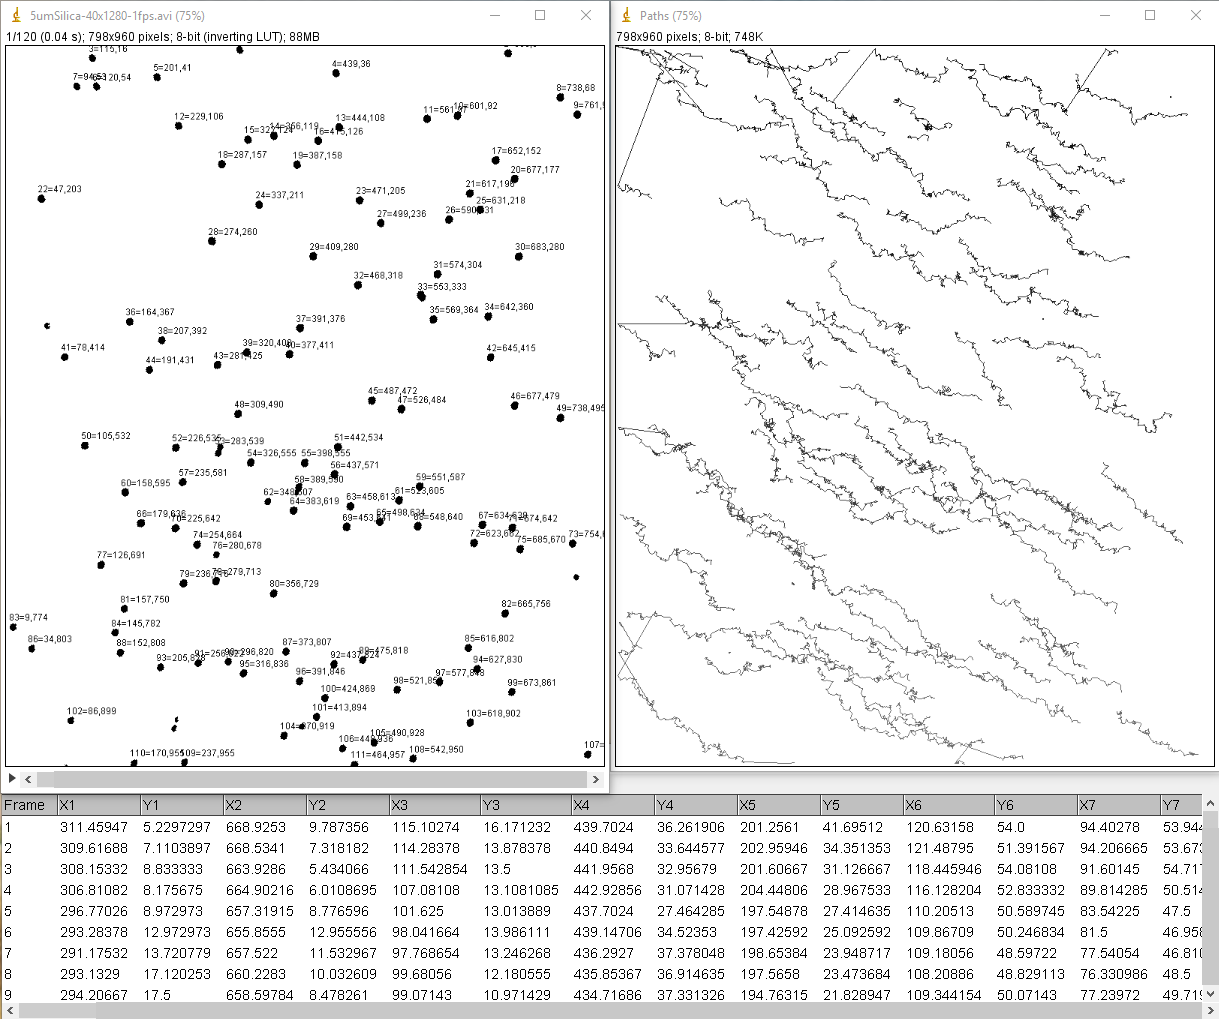
\includegraphics[width=\linewidth]{multitracker}
	\caption{Example Multitracker analysis of microsphere motion}
	\label{fig:multitracker}
\end{figure}

\paragraph*{Characterize the random motion of the beads in your videos.} Compare and contrast their motion to what you would expect for directed motion.
\begin{itemize}
\item Do the average total $x-$ and $y-$ displacements of the beads, $\left \langle \Delta x \right \rangle$ and $\left \langle \Delta y \right \rangle$, change throughout the time intervals you observed? If so, how do they change; if not, why don't they change?
%\item How do the individual total $x-$ and $y-$ displacements of the beads, $\Delta x$ and $\Delta y$, change throughout the time intervals you observed? [\textit{Hint: Make some histograms!}] If so, how do they change; if not, why don't they change? How are these individual displacements linked to the average displacements?
\item How does the total displacement of a particle, $r=\sqrt{\Delta x^2+\Delta y^2}$ , change as a function of the measurement time interval?
\end{itemize}
%
%\begin{table}[ht]
%\centering
%\begin{tabular}{|p{4.5cm}|p{3cm}|p{3cm}|p{3cm}|}
%\hline
% \textbf{Group \# (Parameter)} & \textbf{Video 1} & \textbf{Video 2} & \textbf{Video 3}  \\
% (each parameter will be investigated by two distinct groups, allowing you to `double check' the results) & (condition for testing r$^2$ vs.\ t dependence) &  & \\ \hline
% \textbf{1 \& 2 (bead size)} & 2 $\mu$m silica beads in water & 5 $\mu$m silica beads in water & 1 $\mu$m silica beads in water \\ \hline
% \textbf{3 \& 4 (fluid viscosity)} & 2 $\mu$m silica beads in water & 2 $\mu$m silica beads in low viscosity glycerin/water mix & 2 $\mu$m silica beads in high viscosity glycerin/water mix \\ \hline
% \textbf{5, 6, \& 7 (bead mass \& viscosity)} & 2 $\mu$m PS beads in water & 2 $\mu$m PS beads in low viscosity glycerin/water mix & 2 $\mu$m PS beads in high viscosity glycerin/water mix \\ \hline
%\end{tabular}
%\caption{Video Summary}
%\label{tab:exp3video}
%\end{table}
%
\begin{table}[ht]
\centering
\begin{tabular}{|c|p{1.5cm}|p{2.4cm}|c|c|c|}
\hline
\textbf{Group} & \textbf{Frame Rate} & \textbf{Parameter} & \textbf{Video 1} & \textbf{Video 2} & \textbf{Video 3} \\ \hline
\textbf{1} & 30 fps & \multirow{2}{2.4cm}{\textbf{Bead Size}} & \multirow{2}{2.3cm}{2 $\mu m$ silica in water} & \multirow{2}{3cm}{5 $\mu m$ silica in water} & \multirow{2}{3cm}{1 $\mu m$ silica in water} \\ \cline{1-2}
\textbf{2} & 1 fps &  &  &  &  \\ \hline
\textbf{3} & 30 fps  & \multirow{2}{2.4cm}{\textbf{Fluid Viscosity}} & \multirow{2}{2.3cm}{2 $\mu m$ silica in water} & \multirow{2}{3cm}{2 $\mu m$ silica in low viscosity} & \multirow{2}{3cm}{2 $\mu m$ silica in high viscosity} \\ \cline{1-2}
\textbf{4} & 1 fps & & & & \\ \hline
\textbf{5} & 30 fps & \multirow{2}{2.4cm}{\textbf{Bead Mass \& Viscosity}} & \multirow{2}{2.2cm}{2 $\mu m$ P.S. in water} & \multirow{2}{2.8cm}{2 $\mu m$ P.S. in low viscosity} & \multirow{2}{3cm}{2 $\mu m$ P.S. in high viscosity} \\ \cline{1-2}
\textbf{6} & 1 fps & & & & \\ \hline
\end{tabular}
\caption{Video Summary. `Low viscosity' refers to a 15\% glycerin/water solution, and `high viscosity' refers to a 30\% glycerin/water solution.}
\label{tab:exp3video_v2}
\end{table}

\paragraph*{Plan your analysis.} Use the `Leading a discussion' time to determine, as a class, the best way to analyze your data that allows you to characterizing diffusion.
At the end of the second day of the experiment,  everyone will distribute their data to the rest of the class.
Therefore, make sure that your data files are easy to follow, and that your graphs look professional.

%Day 2
\section{Measuring \& Analyzing Random Motion}
At the end of the first day of this experiment, during the post-experiment discussion, your TA provided you with some information about the Diffusion Constant. 
Begin your second day of this experiment by completing your analysis of video 1 using the plan that you decided as a class would be the best way to characterize diffusion.
Then capture and analyze videos 2 and 3.
\begin{enumerate}
\item \textbf{Examining Diffusion for Video 1:} Does the diffusion constant, D, depend on the measurement time interval (i.e., is D frame rate-dependent)? Using the information you have already created for your first video, investigate how the square of the average bead displacement, $r^{2}$, changes for different measurement time intervals, $\Delta t$. What is the diffusion constant for your video 1?
\item \textbf{Collecting Data for Videos 2 and 3:} These videos have been carefully chosen so that the class, as a whole, can make statements about how varying specific parameters affects the diffusion constant. The parameters of the videos that you capture (i.e., the frame rate, resolution, length, etc.) should be based on what you decided to do as a class at the end of the first day. 
\item \textbf{Analyzing Videos 2 and 3:} Analyzing this data will allow you to combine your results with other groups' work and make claims about how varying the investigated parameter affects the diffusion constant. As with video 1, you will want to analyze these videos according to the plan you came up with as a class. Make a back-up of your data before you begin. Also, make a plan for how to manipulate your data BEFORE you do any calculations in your spreadsheet. (Planning now saves time later!)
\item \textbf{Coordinate with fellow groups.} If you measured the same parameters as another group, meet with them and combine your data before it is sent to the other groups.
\end{enumerate}

\paragraph*{Review your analysis.} Use the `Leading a discussion' time to determine, as a class, if the methods you decided on at the end of the first day are properly characterizing diffusion. If any changes need to be made, work to re-do the analysis before the end of this class. 

%Day 3
\section{Characterizing Random Motion and the Diffusion Constant}
Over the last two weeks, you fully characterized the random motion of beads in fluid and began to determine how changing one parameters of the solution (beads in fluid) can affect the diffusion constant.
In this final week of the lab, you will combine your results with those from the rest of the class, and determine how other parameters of the bead solutions will affect the diffusion constant.
\emph{The data collected by all groups should be included in your lab report.}

\begin{enumerate}
\item \textbf{Examine Diffusion:} Using the data that all of the lab groups have collected over the course of this lab, you are expected to make an argument for a plausible expression for the diffusion constant, D, as a function of some (or all) of the following parameters: fluid viscosity, bead size, and bead mass. (An argument should contain a Claim, Data, and a Warrant—i.e., an explanation of how the claim is related to the data.) You should confirm that this mathematical model for D is plausible by performing a dimensional analysis.
\end{enumerate}

\paragraph*{Things to consider including in your lab report:} As you know, what goes into your lab report should be determined by the ideas necessary to explain and support your work—in designing the experimental protocol, in collecting and analyzing your data, and in forming your conclusions. Here are a few questions you might consider answering:
\begin{itemize}
\item What characteristics have you observed for random motion? (How would these characteristics be similar or different for directed motion?)
\item If the average total displacement in either the x- or the y-direction is zero for all times, why is the displacement NOT zero? How does the displacement change with time?
\item What is the mathematical model that you have constructed for the diffusion constant, D? How is this justified by your experimental data? Do the dimensions work out?
\item How could we design an experiment to find the exact form for the diffusion constant (i.e., how could we figure out the numerical constants that accompany the scaling of D with bead mass, bead radius, viscosity, and temperature)?
\item What could you have done better in your own design and analysis?
\item How are these ideas of random motion and diffusion constants related to (important in) other scientific disciplines?
\end{itemize}

%\begin{table}[h]
%\centering
%\begin{tabular}{|c|p{1.5cm}|p{2.4cm}|c|c|c|}
%\hline
%\textbf{Group} & \textbf{Frame Rate} & \textbf{Parameter} & \textbf{Video 1} & \textbf{Video 2} & \textbf{Video 3} \\ \hline
%\textbf{1} & 30 fps & \multirow{2}{2.4cm}{\textbf{Bead Size}} & \multirow{2}{2.3cm}{2 $\mu m$ silica in water} & \multirow{2}{3cm}{5 $\mu m$ silica in water} & \multirow{2}{3cm}{1 $\mu m$ silica in water} \\ \cline{1-2}
%\textbf{2} & 1 fps &  &  &  &  \\ \hline
%\textbf{3} & 30 fps  & \multirow{2}{2.4cm}{\textbf{Fluid Viscosity}} & \multirow{2}{2.3cm}{2 $\mu m$ silica in water} & \multirow{2}{3cm}{2 $\mu m$ silica in low viscosity} & \multirow{2}{3cm}{2 $\mu m$ silica in high viscosity} \\ \cline{1-2}
%\textbf{4} & 1 fps & & & & \\ \hline
%\textbf{5} & 30 fps & \multirow{2}{2.4cm}{\textbf{Bead Mass \& Viscosity}} & \multirow{2}{2.2cm}{2 $\mu m$ P.S. in water} & \multirow{2}{2.8cm}{2 $\mu m$ P.S. in low viscosity} & \multirow{2}{3cm}{2 $\mu m$ P.S. in high viscosity} \\ \cline{1-2}
%\textbf{6} & 1 fps & & & & \\ \hline
%\end{tabular}
%\caption{[Possible video summary for next semester.] Video Summary. `Low viscosity' refers to a 15\% glycerin/water solution, and `high viscosity' refers to a 30\% glycerin/water solution.}
%\label{tab:exp3video_v2}
%\end{table}
%
%\subsection*{Equipment}
%Familiarize yourself with the Microscope Basics Technical Document before beginning any experimentation. 
%If you do not know how a particular part of the microscope works, please ask your TA — the equipment is expensive! 
%Please be especially careful handling liquid samples near the microscope objectives. 
%\par
%The CCD camera attached to the microscope will allow us to capture video of what we observe. 
%Using the same VirtualDub software we utilized in previous weeks, we can capture AVI videos of the motion we are trying to analyze. 
%In VirtualDub, the microscope camera can be found under `Device' and is named ``ToupCam (DirectShow)''. 
%\par  
%The adjustment options for the microscope CCD camera are slightly less user friendly than the webcam options. 
%However, they are still found in the same VirtualDub menus. 
%Be sure to take note of at which resolution you record your videos; it will be important when determining the distance to pixel ratio. 
%This can be done by taking a picture of the 1 mm calibration slide at the same resolution and magnification level as your videos. 
%If calibration slides are not available, pictures can be found on the lab computers. 
%\par 
%Brightness, contrast, and other exposure settings can be found under `Video' and `Capture Filter'. 
%The most important difference from the webcam cameras is that the frame rate cannot be directly set before capturing videos. 
%It is necessary to control the frame rate by controlling the exposure time of the CCD camera. 
%By telling it to expose the CCD to light for 100 ms intervals, for instance, you are telling it to take a picture every 0.1 seconds.
%This also means that you have to carefully control the amount of light through your sample using the iris and bulb power control. 
%If you are having trouble getting the light settings correct, you can use the Auto Exposure option, but this will often result in very low frame rates.
%
%Since all three videos have captured random motion, we need only look at one video to begin characterizing the behavior of random motion. 
%(Also, you may learn tricks and ideas that can help you analyze the other videos in the coming weeks. Next week, we will teach you automatic tracking!) 
%The method you use to harvest the data is a bit different from what you have done previously with ImageJ. 
%Rather than tracking each object of interest through EVERY frame of the video, we can take very specific frames (reducing the number of clicks you need to make). 
%So, for the beads that you are tracking, you want an initial position (at t=0, the first frame), a final position (at the last frame), and at least 4 other positions (at specific frames equally spaced between the initial and final frame). 
%This will take some careful planning once you have the video in ImageJ and BEFORE you open the Manual Tracking plugin. 
%To compare these beads with each other (histogram-style), you need to be tracking these beads in the all of the SAME frames. 
%For the first video ONLY, we suggest 40-50 beads should be tracked (so that you can create good histograms). 
%For videos 2 and 3, you can use only 15-20 beads (which should be sufficient for the RMS analysis).
%
%On the final day of class, your group will compile all of this data in your lab report as you discuss the effects that these parameters have on the random motion of particles.
%
%\item \textbf{Give Presentations:} Before finishing your lab reports, you should present your work to your peers for critical evaluation. Being part of a community of scientists means sharing your work (in professional journals, through symposia, and at conference talks and poster sessions) for critical evaluation and revision by the community. To model this important aspect of scientific practice, you will create posters presenting your methods, findings, and conclusions. Highlight the important features of your work, your analysis, and your results. During the presentations, ask other groups about what they have done and do not be afraid to ask challenging questions. Your goal is to understand what they have done and how they can improve their work. When you present your work to them, they should ask the same types of challenging questions of you and your group. This should spark some interesting discussions that you can incorporate into your lab report in the evaluation/critic's section.
%
%This week you will continue to explore this random motion, finalizing your histograms ($\Delta$x, $\Delta$y, and r) at various times for video 1 (2 micron beads in water). 
%When your histograms are finished and you have answered the questions asked in last week's lab document (repeated below), fully characterizing the nature of random motion, you should begin analyzing videos 2 and 3. 
%In order to do this, it might help to have a little more information. 
%\par 
%You will discover, as you build your total RMS displacement histograms, that the average displacement magnitude, i.e.\ the average distance traveled by the beads (let’s call it $\left< r \right>$), deviates from zero: Every bead changes its position by some amount! 
%As you remember, the distance traveled can be calculated as $r = \sqrt{\Delta x^{2}+\Delta y^{2}}$, including only the squares of $\Delta$x and $\Delta$y — which are always positive and so add up to something bigger than zero. 
%This equation indicates that instead of the distance traveled, r, we can measure the square of the distance traveled $r^{2} = \Delta x^{2} + \Delta y^{2}$, also called the Mean Squared Displacement or MSD. 
%This makes the math a bit easier, and r$^{2}$ increases linearly with the measurement time interval, as you will see today. 
%\par 
%The ``diffusion constant,'' D, is defined to be the proportionality constant between the average displacement squared, $r^{2}$, of the diffusing object and the measurement time interval, $\Delta$t, over which the diffusion occurs. 
%There is also a factor of 4 in there (for geometry reasons—a 4 in 2-dimensions, a 6 in 3-dimensions, a 2 in 1-dimension):
%\begin{equation}
%r^{2} = 4 D \Delta t
%\end{equation} 
%
%Table
%\begin{tabular}[bt]{|p{.3\textwidth}|p{.2\textwidth}|p{.2\textwidth}|p{.2\textwidth}|}
%	\hline
%	\textbf{Group \# (Parameter)} & \textbf{Video 1} & \textbf{Video 2} & \textbf{Video 3} \\
%	(each parameter will be investigated by two distinct groups, allowing you to `double check' the results) & (condition for testing r$^2$ vs.\ t dependence) &  &\\
%	\hline
%	1 \& 4 (bead size) & 2 $\mu$m silica beads in water & 5 $\mu$m silica beads in water & 1 $\mu$m silica beads in water \\
%	\hline
%	2 \& 5 (fluid viscosity) & 2 $\mu$m silica beads in water & 2 $\mu$m silica beads in low viscosity glycerol/water mix & 2 $\mu$m silica beads in high viscosity glycerol/water mix \\
%	\hline
%	3 \& 6 (bead mass \& viscosity) & 2 $\mu$m PS beads in water & 2 $\mu$m PS beads in low viscosity glycerol/water mix & 2 $\mu$m PS beads in high viscosity glycerol/water mix \\
%	\hline
%\end{tabular}
\newpage{\blankpage}
\chapter{The Competition Between Brownian Motion and Directed Forces}
\thispagestyle{fancy}
\fancyhead[RE,LO]{Experiment \thechapter}

Much of the first month of Physics 2131 focused on directed motion.
In both the lecture and laboratory portions of the course, we saw that when the forces applied to objects did not vary substantially from moment to moment, the objects accelerated/established motion in one particular direction.
\par
Since then, we have begun to explore situations in which the pushes and pulls from the environment surrounding the object fluctuate rapidly in time — so rapidly that directed motion is no longer observed. 
We describe the motion of objects experiencing this volatile bombardment as ``random'' motion. 
In lab we have been exploring some of the qualitative and quantitative features of this random motion.
\par
While ``random'' motion and diffusion are important mechanisms, they propagate very slowly over long distances. 
Therefore, in many biological processes both random and directed motions are utilized. 
Over the next two weeks we will take a look at situations where both random and directed motion can be observed at the same time. 
We will try to determine the conditions under which one or the other type of motion is dominant.

\paragraph{For this two week lab:} Our overall goal here is to create conditions in which our beads undergo both random and directed motion, and to find a way to characterize that situation. 
You will use beads of different sizes suspended in solution to explore the crossover from random to directed motion as an external force is applied.
We've provided you with metal blocks that allow you to tilt the microscope to a couple of different angles.
Tilting the microscope changes the direction of the normal force exerted by the microscope slide on the beads, allowing gravity to have an effect on the beads diffusing around the surface of the petri dish.
Your goal is to observe the crossover from random motion (where thermal forces dominate) to directed motion (where gravity dominates) and analyze how it depends on the size of the bead.:
\begin{enumerate}
\item Make sure that you understand how to safely operate the microscope, how to capture video with the microscope, and the pixel-to-distance ratio of the microscope camera.
\item Capture your first videos and do a preliminary analysis
\item Discuss as a class the method you plan to use to analyze your videos.
\item Collect three videos according to Table .
\item Analyze all of your videos to characterize the motion of the particles.
\end{enumerate}

\section{Random vs. Directed Motion.}
On the first day of this experiment, begin by determining what setup will best allow you to characterize directed motion. 
You will be using a solution of 5 $\mu$m silica beads in water. 
In order to tilt the microscope, you have been provided a few 3/8'' metal steps that you can use to tilt the microscope. 
Be careful when adjusting the tilt of the microscope! 
Have one member of the group tilt the microscope while another member places the steps under the feet.
\par
Adjust the following aspects of your lab setup until you see a good balance of both directed and random motion:
\begin{itemize}
\item \textbf{Tilt Height:} If the tilt is too low, there won't be enough force on the particles for you to see the directed motion; too much, and gravity will dominate over the random motion. Start at a low tilt and move up until you can just begin to notice directed motion in your videos.
\item \textbf{Frame Rate:} Taking a high frame rate video for a few seconds may not show enough movement for the directed motion to be apparent. Try different `low fps' settings until you find one 
\end{itemize}

\begin{enumerate}
\item Video \# 1: A video of 2 to 5 seconds length with about 10 frames per second would be sufficient. Can you observe directed motion? If so, take a video for a long enough time interval that directed motion is clearly visible. Measuring the position of beads for at least 5 time points, create a plot that shows the dependence of $r^{2}$ on time interval for the beads. (If you are using automatic tracking (multitracker plugin), then use all produced data for all `real'\footnote{
A `real' track exists if the bead being followed: a) does not enter/leave the selected area over the course of the entire video; b) does not merge with or separate from another bead/track over the course of the entire video; c) does not blink in and out of existence; d) does not 'jump' (track number switching beads, causing a major discontinuity in x- and y-pixel locations); and e) exhibits some form of motion (i.e., is not stuck to the slide/chamber).} 
bead tracks—not just 5-10 time points.) Is the dependence of $r^{2}$ on time linear, as it was for the random motion when the microscope was not tilted?
\item Video \# 2: Next, take a sample containing 2 $\mu$m silica beads. Record a video of the bead's motion over the same time interval. Track the beads and plot the dependence of $r^{2}$ on time interval. Can you see the directed motion at all or are the beads merely displaying random motion?
\item Video \# 3: Now record a video of the 2 $\mu$m silica beads' motion over a larger time interval (a minute or two). For the sake of video size, reduce the frame rate to ~1 fps. Track the beads (using 10 to 15 time points) and plot the dependence of $r^{2}$ on time interval. What type of motion is visible now?
\end{enumerate}
\subsection*{Interpretation}
Some questions to consider answering in your lab report:
\begin{list}{-}{}
\item If the motion you are observing in some fluid is entirely random, how would you expect $r^{2}$ to vary as a function of the time interval over which you measure? 
If the motion you are observing in some fluid is entirely directed, how would you expect $r^{2}$ to vary as a function of the time interval over which you measure? 
\item Can a log-log plot help you distinguish between random and directed motion? 
Does the slope of the log-log plot change at all? 
Does the slope clearly indicate random or directed motion? 
\item Is it possible to have a situation where both types of motion occur? 
Which one would ‘win'? 
At what time scales? 
What are the conditions under which the motion of an object appears to be purely random? 
What are the conditions under which the motion of an object appears to be purely directed? 
\item Does the concentration of beads that you see on the slide when you look at it under the microscope change at all over the course of the experiment? 
Can you explain this effect using your results?
\end{list}
%\newpage{\blankpage}
\chapter{Motion and Work in Living Systems}
\thispagestyle{fancy}
\fancyhead[RE,LO]{Experiment \thechapter}
%
%\section{Classifying Motion and Examining Work in Onion Cells.}
%\section*{Introduction}
Plant cells store information, food, and waste in small bubbles called vesicles.
These vesicles are transported throughout cells using a combination of mechanisms.
They move throughout cells utilizing random motion, as we have studied previously.
Diffusion is far too slow a mechanism to transport important materials over long distances though, so cells have developed a series of complex mechanisms for directed motion.
In many cells, motor proteins transport vesicles along pathways framed by cytoskeletal fiber.
One such process involves vesicles being transported by myosin motors along actin filaments.
Another involves kinesin motors carrying vesicles along microtubules.
Directed motion is also observed in a process called cytoplasmic streaming, where the vesicles and other material inside a cell moves due to a fluid flow.

\begin{wrapfigure}{r}{0.5\textwidth}
  \vspace{-20pt}  
  \begin{center}
    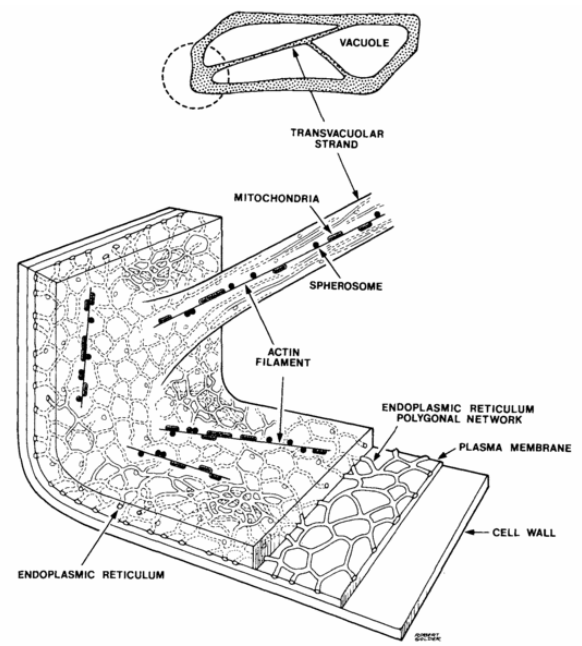
\includegraphics[width=0.48\textwidth]{cellWall}
  \end{center}
  \caption{Inside a cell wall.}
  \label{fig:cell-wall}
  \vspace{-20pt}
\end{wrapfigure}

All of these types of motion can be observed in onion cells.
Therefore, onion cells are a cheap and simple experimental subject that allows us to make several interesting observations.
By looking at individual onion cells, we can make both qualitative and quantitative observations about the different types of motion.
Moreover, analysis of the work required to move the vesicle [based on terminal speed and energy required for ATP hydrolysis (23 kJ/mole), with the step size and efficiency of the motor] can give us insight into the effective viscosity and probable structure of the cytosol (intracellular medium).

\paragraph{For this two week lab:} The goal of this experiment is to understand how quantitative analysis of biological phenomena can provide insight into the structure of living systems. You should aim to capture enough video so that you can fully characterize the motion of around 10 different vesicles. You will use these tracks to model work and power in a physical, living system.
\begin{enumerate}
\item Make sure that you understand how to safely operate the microscope, how to capture video with the microscope, and the pixel-to-distance ratio of the microscope camera.
\item Capture your first videos and do a preliminary analysis.
\item Discuss as a class the method you plan to use to analyze your videos.
\item Collect additional videos if necessary.
\item Analyze your video(s) to characterize the motion of the vesicles.
\end{enumerate}

\subsection*{Investigation}
In order to observe motion inside of individual onion cells, we must first prepare a slide with one layer of onion cells:
\begin{enumerate}
\item Cut down to the center of the onion (activity in the onion cells is dependent on distance from the surface of the onion, thus the center is typically more active). 
\item Once you have a layer of onion close to the center, peel the lower cell membrane off of it( the cell membrane is relatively strong, and is made up of a single layer of cells). 
\item Put a few drops of saline solution down on a slide, place your onion membrane down, and then put a few more drops of saline solution down. 
\item Cover it with a slide cover, and blot the remaining saline solution. 
\item Keep in mind that onions are actually alive, but when you cut into it and mount the membrane on a slide, the cells will slowly die. The lifespan of cells in these slides is around 30 minutes. You might not observe cell activity on the first try; sometimes it will be necessary to try another section of the onion, or even another onion. 
\item Once you have successfully prepared an onion slide, look around to observe all the activity in the cells. You can explore different layers within the cells by changing the focus of the microscope. Most of the interesting activity will be happening at the top or bottom layer of cells. 
\item Find regions where vesicles appear to be moving randomly, and compare them to regions where vesicles appear to be directed somehow. 
\item Take a video or two (be sure to note and record the frame rate for the video) that show both apparently random and apparently directed motion. 
\item Track particles using particle tracking in ImageJ and analyze the two groups of motion using the techniques we have developed so far in the lab. 
\item Before you leave ImageJ, also measure the SIZE of the vesicles (you will need this if you begin working toward the diffusion constant or resistive forces).
\end{enumerate}

\subsection*{Interpretation}
After you have observed the motion both quantitatively and qualitatively, you should be able to make some interesting statements about the motion of vesicles in cells.
\begin{itemize}
\item Is the apparently random motion of vesicles really random or is it confined? Or does vesicle motion look random because vesicles fall off of their ``tracks'' frequently?
\item Where do random motion and active transport occur in cells?
\item How do the velocities of vesicles moving randomly and actively differ?
\item What is the advantage cells gain in utilizing both random motion and active transport of vesicles? When is active transport advantageous, when random motion?
\end{itemize}
Once you have measured the \textbf{average radius} and \textbf{average speed} for the group of vesicles experiencing directed motion, you can do an analysis of energetic concerns to calculate the \textbf{rate of ATP hydrolization} (R) and the \textbf{effective viscosity} ($\mu$) of the cytosol. From the effective viscosity of the cytosol, what can you conclude about the nature and structure of the cytosol? Here are some numbers and equations that might help:
\begin{itemize}
\item Average size of a myosin motor 'step' = 10 nm, stepping along an actin filament.
\item Average size of a kinesin motor 'step' = 8 nm, stepping across/along a tubulin dimer.
\item One 'step' for a motor is equivalent to 1 ATP hydrolization cycle (23 kJ/mole).
\item For both myosin motors and kinesin, the efficiency (work produced $\div$ energy consumed) is 60\%.
\end{itemize}
As you will learn in class shortly, since the vesicle does not change speed, the work being put in (produced by the motor) is being consumed (dissipated) by the viscous resistance within the cytosol.
%With this knowledge, and the following helpful equations, you should be able to determine the effective viscosity of the cytosol and the rate of ATP hydrolysis.
The `efficiency' of a vesicle's motion can be calculated with
\begin{equation}
e = \frac{W_{produced}}{E_{consumed}} = \frac{P_{produced}}{P_{consumed}}
\end{equation}
where W is the work done by the vesicle (in moving itself), E is the energy of one ATP cycle.
This is directly equivalent to the ratio between the power produced and consumed by these entities.
The power consumed by a vesicle can be calculated with
\begin{equation}
P_{consumed} = \frac{N \cdot E}{t} = R \cdot E
\end{equation}
where N is number of ATP cycles, E is the energy of one ATP cycle, t is the time interval. R is the rate of hydrilization.
\begin{equation}
P_{produced} = \frac{F \cdot d}{t} = F \cdot v
\end{equation}
where F is the force generated by the vesicle and d is the displacement.
Displacement divided by time is just the velocity, $v$, of the particles, and can be related to the rate of hydrilization like so:
\begin{equation}
v = \frac{d}{t} = \frac{N \cdot s}{t} = R \cdot s
\end{equation}
where s is the step size.
\par
You also need to consider the viscous force acting on the particles. This can be calculated with \emph{Stoke's Law}, which takes the following form:
\begin{equation}
F_{viscous} = -6 \pi \mu r v
\end{equation}
where $\mu$ is the viscosity, r is the vesicle radius, and v is the speed of the vesicle.
%For comparison, the viscosity of DI water is $8.6 \times 10^{-4}$ Pa$\cdot$s at room temperature (27 $^{\circ}$C).

%For P = Power, W = Work, t = time interval, E = Energy of one ATP cycle, \# = number of ATP cycles, R = rate of ATP hydrolization, e = efficiency, F = force, d = displacement, v = speed of vesicle, s = step size, $\mu$ = viscosity, and r = vesicle radius, the following are true:
\newpage{\blankpage}

\part{Technical Documents}
\renewcommand{\chaptername}{Technical Document}
\renewcommand\thechapter{\Alph{chapter}}
% Edited 8/4/16 EK - full import and correction
\chapter{Introduction to ImageJ}
\thispagestyle{fancy}
\fancyhead[RE,LO]{Technical Document \thechapter}
This year in PHY 2131 we will be using ImageJ for our labs. 
%You may have been exposed to this software through research, internships, or BSCI 205. 
This software is a great tool for use in scientific inquiry. 
Before we teach you how to use it, we think it is important for you to know a little about it. 
ImageJ is an image analysis software developed at the National Institutes of Health (NIH) in 1997. 
Its author, Wayne Rasband, originally wrote it for use by biomedical researchers working with microscope images. 
He designed it with an open architecture so that anyone could write `plugins' to add new tricks to the program. 
As a result, its capabilities are constantly growing and improving. 
Since then, this open-source, Java-based image processing program has become a standard tool for image analysis in many fields, including biology, medicine, radiology, microscopy, etc.
\par 
Depending on what plugins (added program code) are employed, ImageJ can:
\begin{itemize}
\item display, edit, analyze, process, save, and print 8-bit color and grayscale, 16-bit integer and 32-bit images
\item read many image formats, as well as videos and image ``stacks'' (a sequence of image frames sharing the same window)
\item measure distances and angles
\item do geometric transformations such as scaling, rotation, and flips
\item perform standard image processing functions such as logical and arithmetical operations between images, contrast manipulation, convolution, Fourier analysis, sharpening, smoothing, edge detection, and median filtering
\item calculate area and pixel value statistics of user-defined selections and intensity thresholded objects
\item create density histograms and line profile plots
\end{itemize}
Seeing is believing — so rather than engage in a dry discussion of how great ImageJ is and how useful it is in current fields of research, here are a few things you can and should do for yourself:
\begin{enumerate}
\item Visit this website: ``The Cell, an image library'' (\url{http://www.cellimagelibrary.org/}), and look at some of the images produced using ImageJ by scientists around the world. There are video files and still images. It is a searchable database with divisions for Cell Process, Component, Type, and Organism. (Run by the American Society for Cell Biology.)
\item If you are an image analysis/processing junkie, you may want to check out the PowerPoint ``ImageJ, A Useful Tool for Image Processing and Analysis'' (\url{rsb.info.nih.gov/ij/docs/examples/IJ-M&M08.ppt}) created by Joel Sheffield of Temple University. This has lots of information and can give you a feel for the program. We will not use all of these functions in our labs, but it gives you a feel for what ImageJ can do.
\item Check out the list below of some of the scientific poster presentations that were given at the recent ImageJ Conference in Luxembourg. Very cutting edge.
\end{enumerate}
\section*{Selected List of Scientific Poster Presentations at the recent ImageJ Conference, Oct. 2012, Luxembourg}
Links to learn more @ \url{http://imagejconf.tudor.lu/program/start}
\begin{itemize}
\item ``Segmentation and Tracking 4D of C.Elegans early embryogenesis,'' Jaza Gul Mohammed
\item ``Usage of ImageJ program for visualization and analysis of microarray experiments data,'' Denis V. Volkov
\item ``High-throughput Quantification and Analysis of T-Lymphocyte Killing Efficiency with ImageJ,'' Louis Wolf
\item ``Measurement of Nano-particle Uptake in Live Cells using ImageJ,'' Victoria Machtey
\item ``ImageJ in the workflow for generating, evaluating and visualizing 3D gene expression atlas,'' Albina Asadulina
\item ``An ImageJ macro to analyze mitochondrial movement along axon,'' Lai Ding
\item ``Assessment of the surface aspect of foods using ImageJ plugins,'' Lorenzo Fongaro
\item ``Morphometric test-system for patients with ischemic cardiomyopathy,'' Sergey Gutor
\item ``Ultrasonograhic Textural Pattern of Tendon: Analysis with Grey Level Co-occurrence Matrices,'' José Rios-Diaz
\item ``MRE-J: A Novel Pipeline For Magnetic Resonance Elastography Image Processing Using ImageJ and Apache Commons-Math,'' Eric Barnhill
\item ``Using ImageJ to assess radiographic and ultrasound digital images,'' Stefan Andrei
\end{itemize}		%A
%\newpage{\blankpage}
% Edited 8/4/16 EK - full import and correction
\chapter{How to use ImageJ}
\thispagestyle{fancy}
\fancyhead[RE,LO]{Technical Document \thechapter}

\section{Basic ImageJ tasks}

\subsection*{Opening an image}
To open an image, either:
\begin{itemize}
\item Click `File $>$ Open', and then navigate to the image you wish to analyze.
\item Drag and drop the image you wish to analyze onto the main ImageJ window.
\end{itemize}
To open a video file:
\begin{itemize}
\item Click `File $>$ Import $>$ AVI...'. Select the video you wish to import then click `Okay'.
\item In the `AVI Reader' window that opens, select the `Convert to Grayscale' option, and click `Okay'.
\end{itemize}
After importing a video file, you may need to edit it in order to allow our tracking tool to properly follow different features.
\begin{itemize}
\item Once you have selected an appropriate area, highlight this area with the *Rectangle* selection tool, click on `Image $>$ Crop'. 
This will delete the rest of the video, and leave only the relevant section. 
If you want, you can use the zoom button (`Ctrl + ``+''') to make this selection a bit larger on your screen.
\item Now that we have an appropriate video, we need to process it to the point of being black features on a white background, with limited noise. 
The first step is set the threshold for the video, which basically takes all of the shades of gray in the video and turns it into black or white. 
To do this:
\begin{itemize}
\item Click on `Image $>$ Adjust $>$ Threshold'. 
\item In the menu that pops up, play with the sliders until the featrures you are investigating are displayed in black, but there is no black elsewhere in the video. 
It should look similar to the screenshot. 
\item Once you have achieved this, click on the apply button. 
Apply the threshold to all of the frames of the video, but you don't have to calculate it each time, the first is enough. This should produce images similar to the one in the screenshot, with black spots on a white background.
\end{itemize}
\item You may notice that there are some little spots of noise around your images. 
To fix this:
\begin{itemize}
\item Go to `Image $>$ Adjust $>$ Contrast'.
\item Set the contrast tab all the way to the right.
\item This should further separate the difference between black and white, leaving just the black spots of the beads
\end{itemize}
\end{itemize}
\subsection*{Determining distance-to-pixel ratio in ImageJ}
Once you have imported a file into ImageJ, you will need to determine the distance-to-pixel ratio for your video (this should be done separately for each image/video analyzed). 
\begin{itemize}
\item You will need to use the `line' tool (*Straight* tool, 5th from left end of icons in toolbar) in ImageJ.
\item Click on the `line tool' icon of the ImageJ menu toolbar (it looks like a sloped line or a slanted fraction bar (/), and the bottom right corner has a downward-pointing black triangle). 
\item Using this tool, click on one end of a `known length’ object hold down the mouse button, and drag the line across the `known length’ object to the other side. 
\item Click `Analyze $>$ Set Scale...'. Edit `Known Distance' and `Unit of length'. Now that the scale is set, the rest of the measurements that you take will be reported in the entered units.
\end{itemize}

\section{How to use ImageJ automatic tracking}
The main difference between manual and automatic tracking is the preliminary image processing that is required. 
It takes longer to prepare each video for analysis, but automatic tracking makes it much easier to quickly track many particles. 
Essentially, our goal will be to process our image sequence to the point where our particles appear as black spots on a white background.

\subsection*{Gathering Data with the Automatic Tracking Plugin}
Once you have processed your video, you can open the Automatic Tracking plugin. 
The Automatic Tracking plugin allows you to collect horizontal (X) and vertical (Y) position coordinates for objects at different times within the video automatically by only describing the sizes of the objects you want to look at. 
To activate the Automatic Tracking plugin:
\begin{itemize}
\item Click on `Plugins $>$ 2131\_Plugins $>$ MultiTracker'. A new window will appear. 
\item Adjust the min and max size if necessary to exclude any noise in your video. 
Because of the way we processed the image, the only objects in the video should be the beads we are looking at, so these parameters should work.
\item If you would like a clearer idea of which bead is which, and where they move over time, you can select the Show Label/Path options.
\end{itemize}

\subsection*{Exporting the Automatic Tracking Data to Excel}
When the data collection is finished, go to your data window and examine how many different particles were tracked for the video. 
The columns of the resulting data table will just be the X and Y positions for each of the particles that the computer identifies. 
Make sure that you only use data for real beads displaying real random motion. 
You can check this by identifying the object at each coordinate position in the result table. 
If the computer recognized noise as a bead, make sure you exclude this from your analysis. 
If a bead enters or leaves the screen, make sure you exclude this point as well. 
If a bead is clearly stuck to the slide and not moving at all, you may want to consider excluding that data point. 
Once you are sure that you have identified the beads in your results table, you can save your results into an excel file (Option 2 is best for this, as there will be MANY columns).
\begin{itemize}
\item Option 1: `Edit' $\rightarrow$ `Select All' $\rightarrow$ `Ctrl' + `C' to Copy $\rightarrow$ Paste into an Excel file (you must add the column titles yourself), or
\item Option 2: `File' $\rightarrow$ `Save As...' $\rightarrow$ Name the file what you will and click `Save'. (It will save in Excel format with column titles.)
\end{itemize}	%B
\newpage{\blankpage}
\chapter{Scientific Data Analysis with Excel}
\thispagestyle{fancy}
\fancyhead[RE,LO]{Technical Document \thechapter}
%
Excel (or any spreadsheet program) can help you do calculations quickly and efficiently. 
But Excel is only a software program — it can only be as smart as the instructions that you give to it.
This technical document will walk you through all the basic steps that you will need to use in each experiment to properly analyze your data.
Each version of Excel (as with the other Microsoft Office programs) varies slightly, but familiarity with one version should help you intuitively guess/explore the other versions. 
Some of you may feel that you are already familiar with Excel; please READ this Technical document anyway! 
It contains specific scientific norms that you need to learn.

\section*{Entering Data:}
%\includegraphics[width=\linewidth]{exAn1}
%In a blank/new Excel document:
%\par 
To enter information in a cell, click on the cell (e.g., cell A1—column A, row 1) and type the information. 
When you are finished, press `Enter.' 
You will see the information in the cell. 
To edit the information, click on the cell and type (erases previous entry) or click on the cell and then click on the formula bar to edit (the formula bar is above all the cells but below all the icons for text manipulation (bold, italicize, center in cell, etc.).
\par 
When you are entering data into excel, begin by adding a title to each column with the quantity's name and units.
In the cells beneath each column title, enter the data that you have collected by typing the numbers into the cells.
When you have finished entering your data, save the file by pressing `Ctrl' + `S' (name the file and note the saved location for future use) or by selecting the `File' tab, then the `Save as' icon. 
Save regularly to avoid losing work.
Every time you save the file, it overwrites the previous version.
\par 
The number of decimal places displayed in the cell can be controlled by icons in the `Number' menu on the `Home' tab.
Use these icons to give your data uniform appearance.

\section*{Generating Columns of Data Calculated from a Formula:}
To generate information from a formula (i.e., to mathematically manipulate cells), click on a cell and begin with =. 
All Excel entries for which you expect a numerical result/output MUST begin with an equals sign, =. 
The mathematical manipulators are what you would expect: * to multiply, / to divide, + to add, and – to subtract. 
To exponentiate, type \char`\^ \ and the power (e.g., $6^{2}$ is 6\char`\^2). 
Let's say you wished to multiply the entry in cell A1 by 60. 
To do this you would click on the cell where you wish the output to go and then type:

\medskip
\texttt{=60*A1}
\medskip

You can type the input cell, A1, on the keyboard, or you can use the mouse to click on cell A1 while typing the formula. 
For more complex mathematical operations, parentheses often become necessary. 
Excel will color-code the parenthesis to help you see where each set opens and closes. 
Be VERY careful with your parentheses!
(Again, Excel is only as smart as the instructions that you give to it!)
\par 
If you wish the same mathematical formula to be applied to every cell in a column (e.g., column F is column A times 60), type the formula into the output cell for the first row. 
Then click on the output cell and move your mouse over the bottom, right corner of the cell. 
Your pointer will change shape and become a plus. 
Click the left mouse button, drag down to the last cell you wish to effect, then release the mouse button (you can also double click the bottom left corner). 
The cells will automatically fill in. 
By clicking on any of these cells, you can see in the formula bar that the formula has been adjusted to reference the correct input cell (i.e., for the row you are currently in). 
The same process can be used to copy a formula across a row into multiple columns. 
If, in a formula, you wish to reference a specific column or cell (that will NOT change when the formula is dragged over a column or row), use the \$ symbol: e.g., \$A1 will always be column A, but the row number can change; and \$A\$1 will always be column A and row 1 — neither can change. See the example below in figure \ref{fig:exc1}:

\begin{figure}[ht]
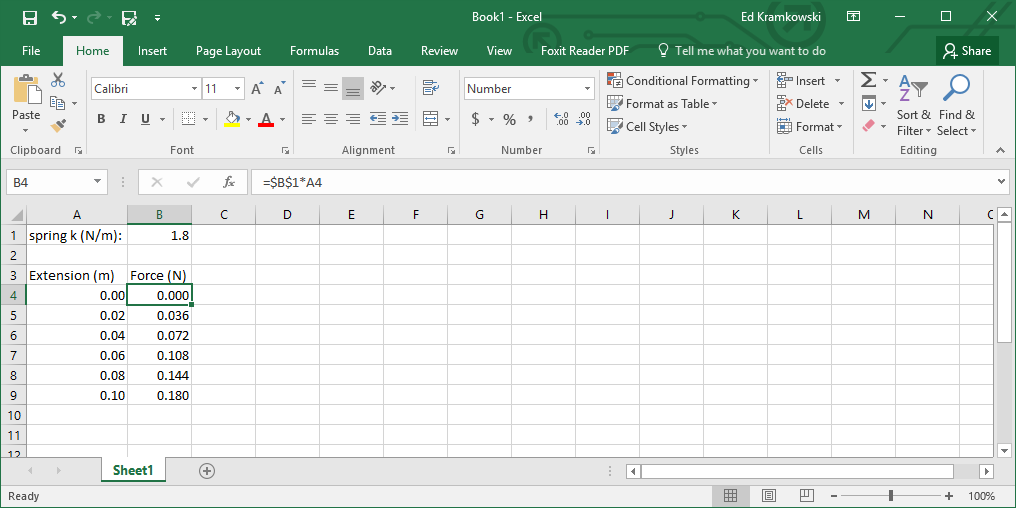
\includegraphics[scale=0.5]{excel1.png}
\centering
\caption{An example of using the \$ symbol to use a constant in a calculation. The force of a spring is calculated using $F=k * x$, where k is the spring constant and x is the extension of the springs length.}
\label{fig:exc1}
\end{figure}

Another example is shown in figure \ref{fig:exc2}, which is in the last section of this technical document.

\begin{figure}[ht]
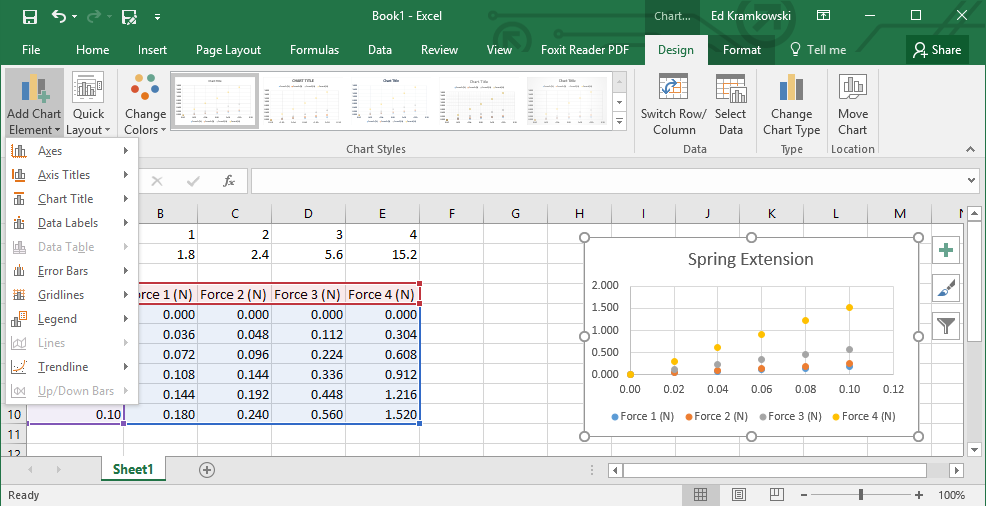
\includegraphics[scale=0.5]{excel4.png}
\centering
\caption{To add other elements to your chart (e.g. axis titles), choose ``Add Chart Elements'' from the ``Design'' menu.}
\label{fig:exc4}
\end{figure}

\section*{Generating Graphs:}
When creating a graph/plot, Excel will usually plot the first column on the independent/ horizontal axis and the second column on the dependent/vertical axis. 
You should always check that the correct data has appeared on the correct axis. 
If the data has been entered with the columns in reverse order, this can be fixed after the plot is created.
\par
To generate a graph/plot, use the mouse to highlight the data that you wish to graph (if the data is adjacent, just highlight the entire chunk; if the columns are not adjacent, highlight each column separately while holding the `Ctrl' key). 
Once the data is highlighted, click on the `Insert' tab and then the `Scatter' icon (on the `Charts' menu - other types of charts may be appropriate for different data types, but the Scatter plot is the most commonly used). 
From the sub-types of scatter plot available, choose the one that has data points but no lines. 
A graph will appear — but you are NOT finished yet!
\par
The design of the graph can be adjusted using the `Chart Layout' menu (see figure \ref{fig:exc4}) - you will want to be able to label the individual axes with the quantity graphed and its units and you will want to be able to title the graph. 
When the graph has been titled (for the `vs.' format, it is always `Dependent' vs. `Independent') and the axes have been properly labeled, you can choose to keep or delete the Legend (not needed if only one data set is plotted, absolutely necessary for multiple data sets). 
The location of the chart can be changed by: left-clicking on the chart (the upper right corner works well), then right clicking and choosing `Move Chart' from the menu. 
It is often best to make the chart a `New Sheet' (so that it doesn't block your view of the data) - give it an appropriate title and click `Okay.' 
You chart will become its own sheet - and your data will disappear! 
But the data is not gone - to find it, use the tabs on the bottom of the Excel window (`Sheet 1' is usually the data; now might be a good time to rename it `Data': right click, select `Rename' and name it).
\par 
Before you finish, check that the correct data has been plotted on the correct axis and that the axis labels match the quantities plotted (see figures \ref{fig:exc5} and \ref{fig:exc6}). 
If the original columns were in reverse order, this can be adjusted by left-clicking on a data point (to select the data), and then right-clicking and choosing `Select Data.' 
Click on the Legend Entry you wish to adjust, and then click `Edit.' 
Highlight the appropriate Series X and Series Y data and then click `Okay.'

\section*{Making Good Graphs}
One thing you should focus on in this class is developing good graph-construction habits.
Presenting data in a graph that is both accurate and easy to follow is an important skill to have in any scientific discipline. \\
When formatting your graphs:
\begin{itemize}
\item Give your graph a descriptive title.
\item Make sure that all axes are labeled at a legible font size; do not forget to include units.
\item If you are graphing discrete data points (as will be the case most often), use only the basic scatter plot.
\item If your graph contains multiple independent data sets, be sure to include a legend.
\item Include a caption giving a short description of your graph. Make sure to note any important features.
\end{itemize}
\begin{figure}[ht]
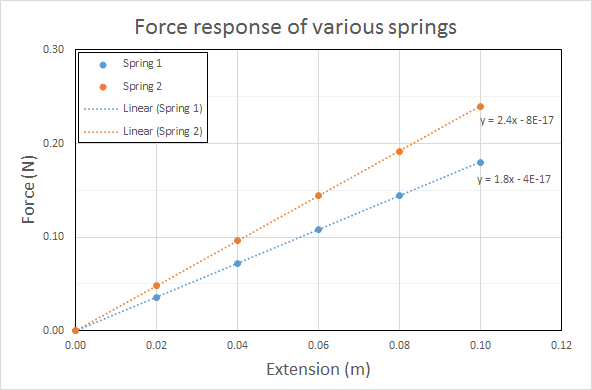
\includegraphics[scale=0.5]{excel3.png}
\centering
\caption{An example of properly graphed data.}
\label{fig:exc3}
\end{figure}

\section*{Adding a Best Fit (``Trendline'') to a Graph:}
To add a line of fit (called a ``Trendline'' in Excel) to a graph, left-click on a data point to select the data, then right-click and choose `Add Trendline.' 
Choose the appropriate Trend/Regression type, and tick the boxes for `Display Equation on chart' and `Display R-squared value on chart.' 
As a general rule, do not `Set Intercept' to a specific number (i.e., do not force the origin to be part of the trendline). 
Do you know what the R-squared value really means? 
If not, you should look it up! 
Look at the equation for the trendline and think about it. 
What does the slope mean? 
What does the y-intercept mean? What does this R-squared value mean?

\section*{Adding Error Bars to the Data Points on a Graph:}
Error bars represent the uncertainty of the measurement of the data. 
Do you have uncertainty? 
Do you have uncertainty in both quantities (horizontal and vertical)? 
Is the uncertainty the same for all data points, or does it change with the value of the quantity plotted? 
Wherever you have uncertainty, you must have error bars! 
Once you have determined the amount of uncertainty, you can add error bars by clicking `Add Chart Elements' inside the `Chart Tools' tab. 
Select `More Error Bars Options', then select the data set that you are adding error bars too.
This should open up the format window, which will allow you to select the length of the error bars (under `Error Amount').
Apply the error bars according to the decisions that you have made about your uncertainty; a good choice is often `Standard Error', but you may sometimes wish to use errors that you calcuated by selecting `Custom' and then selecting the appropriate columns with your errors. 
To remove either vertical or horizontal error bars, left-click on the bars, then right-click and choose `Delete'.

\section*{Other cool tools:}
As a spreadsheet program, Excel can do a lot of useful statistical analysis and mathematical manipulation. 
Some functions you will find useful include: Sum, Average, and Standard Deviation.
\par 
To \textbf{Sum} elements, click on the cell in which you wish the result to appear, then enter \texttt{=sum}. 
Immediately, Excel will list possible formula options that begin with \texttt{sum}. 
For a simple summation of elements, you would choose the SUM function, which you have already typed, but you should note the other options available. 
Open parentheses following your sum, so that you have now types \texttt{=sum(} and then highlight the cells to be summed. 
Close your parentheses and press `Enter.' 
(It would look like this \texttt{=sum(A1:A5)} for a sum of the cells in rows 1 through 5 of column A.)
\par 
To \textbf{Average} elements, click on the cell in which you wish the result to appear, and then enter \texttt{=average(}. Highlight the cells you wish to average and then close your parentheses and press `Enter.' 
Note that Excel will offer you a list of average functions - the most commonly used option is the AVERAGE function. (It would look like this \texttt{=average(A1:A5)} for the average of the cells in rows 1 through 5 of column A.)
\par 
To perform a \textbf{Standard Deviation} on a set of elements, click on the cell in which you wish the result to appear, and then enter \texttt{=stdev.s(}. 
Highlight the cells you wish to perform a standard deviation upon and then close your parentheses and press `Enter.' 
Note that Excel will offer you a list of standard deviation functions - the most commonly used option is the STDEV.S function. 
(It would look like this \texttt{=stdev.s(A1:A5)} for the standard deviation of the cells in rows 1 through 5 of column A.)
\par 
To perform any of these functions on disconnected sets of cells (e.g., cells in rows 1 through 13 and then 15 through 17), open your parentheses, highlight the first contiguous group, enter a comma, then highlight the next contiguous group, enter a comma, and so forth, continuing to the last group of numbers and ending with a closing parenthesis and the `Enter' key. 
(As an example, \texttt{=average(A1:A13,A15:A17)}.)
\par 
Excel has many other functions available, including trigonometric and logarithmic functions. 
Investigate what is available by clicking on the `Formulas' tab and looking through the `Function Library,' especially the `Math \& Trig' and `More Functions' menus.

\section*{Other Examples}

\begin{figure}[ht]
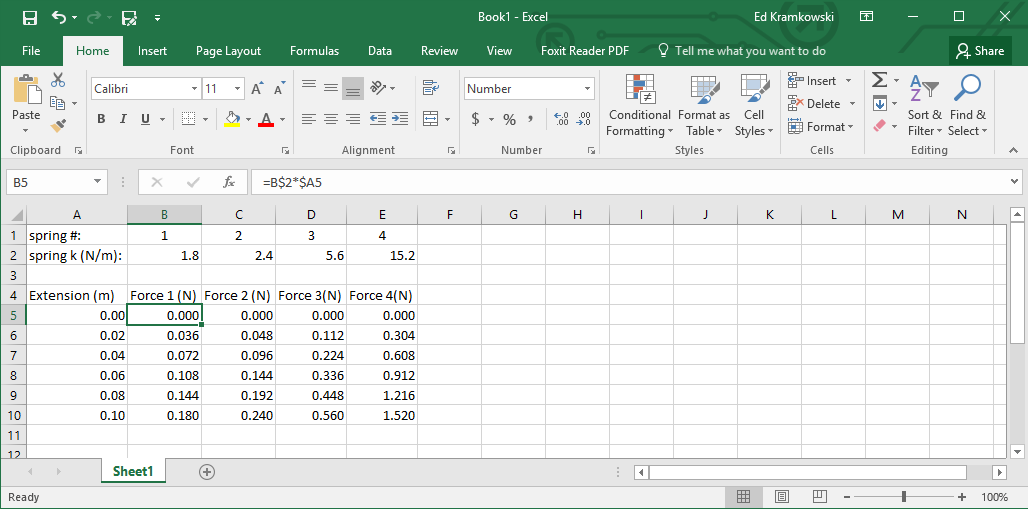
\includegraphics[scale=0.5]{excel2.png}
\centering
\caption{Another example of using the \$ symbol to use a constant in a calculation. By typing the formula \texttt{=B\$2*\$A5} into cell B5, you can allow the constant to change along a specified axis, while continuing to multiply by the numbers in the `Extension' column.}
\label{fig:exc2}
\end{figure}

\begin{figure}[ht]
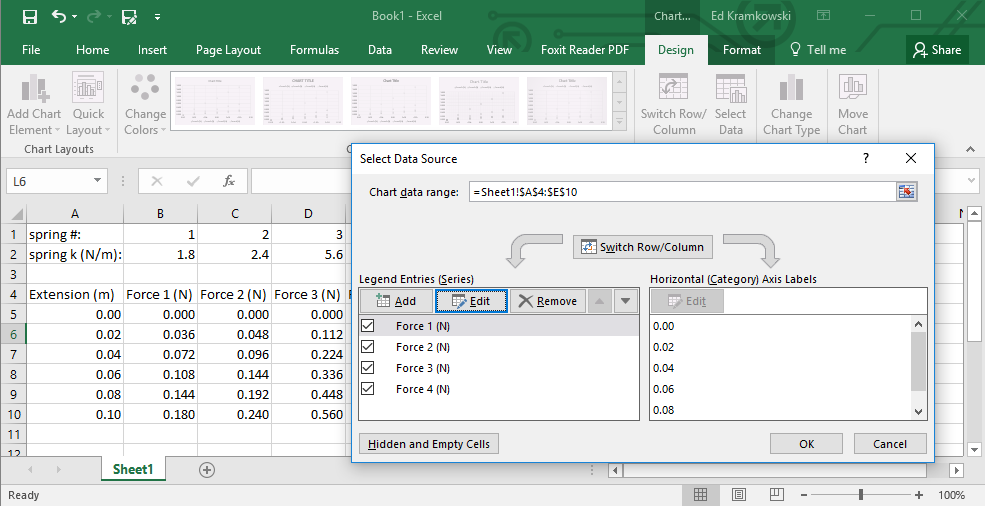
\includegraphics[scale=0.5]{excel5.png}
\centering
\caption{To edit or add sets of data to a graph, choose ``Select Data'' from the ``Design'' menu.}
\label{fig:exc5}
\end{figure}

\begin{figure}[ht]
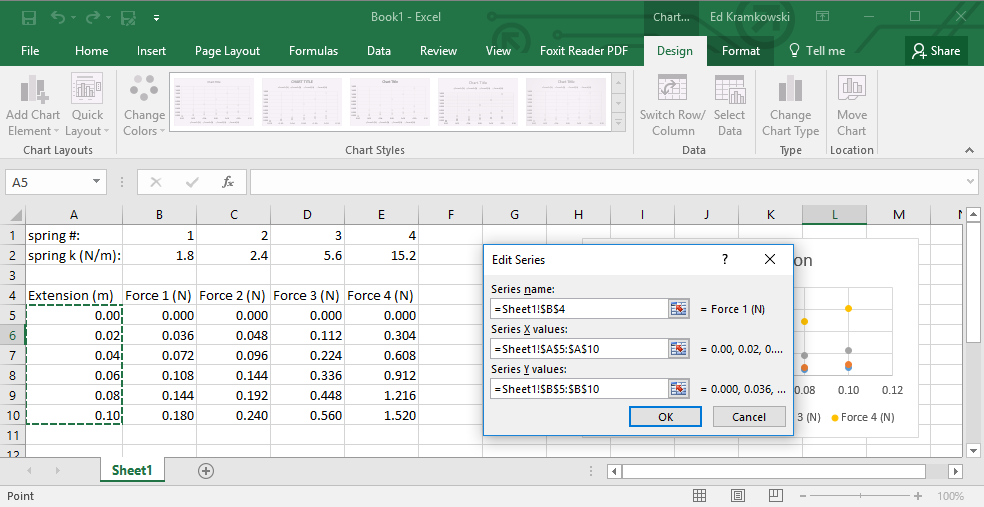
\includegraphics[scale=0.5]{excel6.png}
\centering
\caption{After selecting ``Edit'' in the ``Select Data Source'' menu, you can check if the values are being graphed on the proper axes, and edit the size of the data series if necessary.}
\label{fig:exc6}
\end{figure}	%C
\newpage{\blankpage}
\chapter{Creating Histograms in Excel}
\thispagestyle{fancy}
\fancyhead[RE,LO]{Technical Document \thechapter}
There is more than one way to do this!
We will present two ways:
\begin{itemize}
	\item Option \# 1: Using the Histogram Tool in the Data Analysis Package, and
	\item Option \# 2: Using the Frequency Function.
\end{itemize}
Choose whichever works best for you, given the settings available in your version of Excel.
%
\section{Using the Histogram Tool in the Data Analysis Package}
Excel has several `Add-Ins' that can be activated for the `Quick Access Toolbars.'
To see if the Data Analysis Add-In is activated on your version of Excel, click on the `Data' tab and look for this AddIn in the `Analysis' portion of the toolbar. 
(If it is not activated, you can try activating it by using the following steps: Position mouse over the `Data' tab and right-click; select `Customize Quick Access Toolbar...;' click on `Add-Ins;' Select Manage `Excel Add-Ins' and click `Go;' check the Analysis ToolPack and click `OK;' agree to activate the Add-In.
Now you should see the Data Analysis Add-In in the Analysis portion of the Data tab.)
\paragraph{Step 0: Make a plan!} 
Always have a plan in mind before you ask Excel to do anything! 
Looking at the full range of the data you wish to histogram, decide on a reasonable number of equal-sized bins and figure out what the boundaries of these bins should be. 
Type these boundaries into a column in Excel. 
(For example, if we histogram test grades, we might select bins ranging from 0 to 100 points, with 10 bins, each 10 points large. Here the bins are 0-10, 11-20, 21-30, 31-40, 41-50, ... 81-90, 91-100. These bin `boundaries' are 0, 10, 20, 30, 40, 50, ... , 90, and 100.)
\paragraph{Step 1: Activate the Histogram Analysis Tool.} 
Find the Data Analysis Add-In and click on it. 
Choose the `Histogram' analysis tool and click `OK.' Select the data you wish to create a histogram of and put this into the `Input Range' box. 
If you have decided what the boundaries of your bins will be, select the boundaries and put this into the `Bin Range' box. 
(If you don't enter anything into the Bin Range box, Excel will calculate these on its own — but, as we know, Excel does not always make good choices when left alone!) 
Click the `Output Range' bubble and enter a cell in your spreadsheet (this is where the results from the Histogram tool will be displayed). 
Then click `OK' and the analysis will be run.
\paragraph{Step 2: Understand the Histogram Output.} 
The Histogram analysis tool will output both Bin and Frequency data. 
An Example of such output is given here. 
The Frequency indicates the number of items from your data that fell between the previous and the current bin; i.e., a Frequency of 16 for Bin 10 says that the data you analyzed fell between the values of 5 and 10 a total of 16 times. 
The Bin `More' represents the number of times the data you analyzed has a value more than your maximum bin boundary; i.e., a Frequency of 0 for the More Bin indicates that none of the data you analyzed had a higher value than 25.
\paragraph{Step 3: Create the Histogram Plot.} 
Now you just need to make a bar graph of this data. 
Highlight the frequencies and click on the `Insert' tab, then click `Column' and select `2-D Column.' 
To adjust the horizontal axis labels, click on the plot, right click, and choose `Select Data,' then choose to edit the Horizontal Axis Labels. 
Title and label the plot appropriately. Tada!
%
\section{Using the Frequency Function}
Suppose you want to produce a histogram showing the distribution of student grades on a recent exam. 
The following guide outlines the procedure you would need to follow. 
\paragraph{Step 1:} Scan your data to get a sense for the overall range of values. 
For our example, the grades fall between 50 and 100, so this is the range that our bins must span. 
The next decision is how fine you want the increment of your bins to be — the finer the increment, the more bins, and thus the more bars in our histogram. 
For our sample data set, a bin increment of 10 seems appropriate. 
Create a column next to the raw exam score data that shows the bin ranges, and a column to the right of that which shows the maximum values of your bins. 
\paragraph{Step 2:} Now use the Excel function FREQUENCY to determine how many values fall within each of the bins that you have defined. 
The FREQUENCY function is an array function, returning values to a range of cells. 
Follow the following steps to enter the FREQUENCY function:
\begin{itemize}
\item Highlight the range of cells which will hold the frequency counts (E2:E7). These will be all of the Frequency Count cells next to the max bin values.
\item Choose Insert $>$ Function..., pick the Statistical Function category and scroll down in the box on the right and choose FREQUENCY as the Function name.
\item Use the dialogue box to enter the function. With the Data\textunderscore array box selected, go to the spreadsheet page and highlight the data values (A2:A17). The dialogue box with ``roll up'' while you highlight these values and then ``roll down'' when you are done.
\item Repeat this process by selecting the Bins\textunderscore array box and then go out the spreadsheet and highlight the bin limits cells (D2:D7).
\item Click OK. The completed formula is seen in the formula bar and the correct count value is seen in the Bin Limit 50 count cell (E2).
\end{itemize}
\paragraph{Step 3:} Now copy the array function down to the other Frequency Count cells. 
This is a bit different than typical cell copying:
\begin{itemize}
\item With the Frequency Count cells still highlighted (E2:E7), click on the FREQUENCY function into the formula bar (i.e., \texttt{=FREQUENCY(A2:A17,D2:D7)}).
\item Propagate the function by typing Control-Shift-Enter on a PC (type Command-Return on a Mac).
\end{itemize}
The frequency values should now fill the cells next to the bin increments. 
Note that your first bin increment, 50, holds all the grades at 50 and below. 
The next bin, 59, holds measurements from 50 - 59, and so on.
\paragraph{Step 4:} Create a bar chart plotting the frequency count (Column E) as a function of the student grade increments (Column C).		%D
\newpage{\blankpage}
\chapter{Introduction to Video Capture}
\thispagestyle{fancy}
\fancyhead[RE,LO]{Technical Document \thechapter}
\section*{Finding the software on the lab computer}
The software should be clearly available on the desktop. 
If it is not, go to the start menu and type `virtual' into the Search Programs and Files box. 
The software you want is called `VirtualDub' and has an icon that looks like a gray gear-and-screw. 
Open this.
\section*{Capturing video with the webcam}
Select `File $>$ Capture AVI' to get the webcam activated. 
If both a webcam and a microscope are connected to your computer, you may need to select the device. 
Select `Device,' and `Microsoft LifeCam Studio (TM) (DirectShow)' for the webcam or the `UCMOS03100KPA' option for the microscope.
If you do not see the output from the camera showing in the window, make sure that `Video $>$ Preview' is checked.
\par 
To adjust the color space compression, output size (resolution), or frame rate, select `Video $>$ Capture Pin'. 
To adjust brightness, contrast in the image, and other exposure settings, select `Video $>$ Capture Filter'. 
Under the `Camera Control' tab, you may wish to uncheck auto-focus after you experiment is setup, to avoid the camera shifting the focus during a measurement.
These two methods are very important and significantly different for the microscope, and you will learn more about this later. 
\par 
To adjust the length of your video, select ‘Capture $>$ Stop Conditions’. 
Be aware that ImageJ can process only about 400 frames (due to the limited working memory of the computer, more frames possible with the virtual stack option), so you will need to adjust the play rate and total time of your video to take the minimum length to capture your event and not much else. 
\par 
To begin capturing a video, you first need to set a name for the resulting file. 
To do this, select `File $>$ Set Capture File', and input a file name. 
You should be saving your files to different folders for different experiments, so as not to confuse them. 
Create a folder for your group to use in My Documents. 
Then click `SAVE'. 
Also make sure to check `Capture $>$ Autoincrement filename after capture' to avoid accidentally overwriting any of your good data.
\par 
When you are ready to capture video of motion/your subject, select `Capture $>$ Capture video' or press F5. Once your experiment is complete, press `Esc' to stop recording. 
Keep in mind, you may need to collect several trial videos before you manage to get good video for analysis in ImageJ.
\section*{Capturing video with the microscope CCD camera}
Unfortunately, the user interface for the microscope camera is not quite as friendly as the webcam. 
In fact the frame rate, which is very important for the measurements you will be doing, is difficult to set exactly. 
\par 
The capture process for the microscope camera is very similar to the webcam. 
The main difference are in how to set the video settings, such as resolution, frame rate, and brightness. 
To adjust the output size (resolution, select ‘Video,’ ‘Capture Pin’). 
There should be three options available, but keep in mind that higher resolutions lead to drastically larger files. 
To adjust brightness and frame rate, select ‘Video,’ ‘Capture Filter’. 
Because of the nature of the camera, the best way to control the frame rate is to change the exposure time. 
The exposure time value is around the spacing  between frames, so 0.5 s exposure time will translate to around 2fps. 
Changing the exposure time will also change the brightness of the image, as more light will be collected for each frame. 
After you set the exposure time and take a video, it is important to record the resulting frame rate. 
You can find the frame rate in the information panel on the right of the video capture screen, under the video tab and next to the label “average rate.” 
\par 
The remainder of the video capture process for the microscope is identical to the webcam process. 
Be sure to change the name for each video to something that helps you identify the video, and don’t forget to record the frame rate!
\section*{Video construction \& planning}
Creating a good video for analysis in ImageJ is tougher than you might think. 
You will need to consider elements of video construction and planning. 
You need to be a ‘Good Cinematographer.’ 
Here are some questions to consider:
\begin{itemize}
\item What is the best angle? How should the camera be aligned to view the motion of the object
in which you are interested?
\item What is the best time between frames? How many frames-per-second should you be collecting, given the time for the phenomena to occur and the memory limitations of ImageJ (about 400 frames)?
\item Is there a known length visible in the video?
\item Are all objects of interest clearly visible in the video?
\item Is the entire portion of motion in which we are interested visible in the video?
\item Is the camera (perspective) stationary?
\end{itemize}
\section*{Determining distance-to-pixel ratio in ImageJ}
Once you have imported the .AVI file into ImageJ, you will need to determine the distance-to-pixel ratio for your video (this should be done separately for each video analyzed). 
\par 
You will need to use the 'line' tool (*Straight* tool, 5th from left end of icons in toolbar) in ImageJ. 
Click on the 'line tool' icon of the ImageJ menu toolbar (it looks like a sloped line or a slanted fraction bar (/), and the bottom right corner has a downward-pointing black triangle). 
Using this tool, click on one end of a ‘known length’ object hold down the mouse button, and drag the line across the ‘known length’ object to the other side. 
Without releasing the mouse button, look to see the length (in pixels) of your line segment--this information should be at the top of the video window or at the bottom edge of the ImageJ menu toolbar. 
It will say "length=.....". 
This length, in pixels, is equal to the ‘known length’ of the object. 
Now you have a distance-to-pixel ratio to help you turn pixel locations into physical positions. 
Once the mouse button is released, this pixel length will no longer be displayed by ImageJ. 
It can be recovered by selecting ‘Analyze,’ ‘Measure’ and looking at the measurement on the data table that appears.		%E
\newpage{\blankpage}
\chapter{Measurement Error}
\thispagestyle{fancy}
\fancyhead[RE,LO]{Technical Document \thechapter}
%
When getting quantitative information from a measurement, we are interested not just in the value
we obtain, but in how sure we are that the value we have measured is correct.
There are many factors that can produce a shift or an uncertainty in a measurement – we could have a meter stick with the end chipped off, our dials can only be read to a certain number of significant figures so the next digit is uncertain, or the setup conditions for our experiment can't be arranged precisely. 
In standard terminology these are referred to as ``errors'' – though this is a technical term that really means ``uncertainties.'' 
There is no implication that there are any mistakes made in doing the experiment!
Once we have a good estimate of how much uncertainty there is in our measurement, we estimate an error bar – a spread of values that says, ``We expect the odds are 2:1 that the actual value is inside this range.''
\par
Errors like our meter stick being chipped off and thus too short are called systematic errors. 
They always shift the result in one specific direction and need special care to reduce them.
Errors that arise from many small hard to control uncertainties (e.g. how well two fluids are mixed, how stable the temperature of the apparatus is, or whether the measurement is affected by building vibrations) are well studied mathematically and are referred to as random error, and these errors make the result bigger OR smaller in a RANDOM fashion. 
One way to get a handle on this random error is to repeat the experiment a number of times, preparing it as similarly as you can, and see how much variation there is. 
The statistical tools of mean (average) and standard deviation allow you to estimate both the average result and the error bar arising from random error.

\section*{Mean, Standard Deviation, \& Standard Error}
Given a number of measurements of the same event, the best estimate of the measurement is the mean of the values found,
\[ x_{best} = \bar{x} = \frac{1}{n} \sum_{i=1}^{n} x_{i} \]
where $n$ is the number of measurements.

A useful way of characterizing the reliability of the measurements is to calculate the standard deviation,
\[ \sigma = \sqrt{\frac{1}{n-1} \sum_{i=1}^{n}(x_{i}-\bar{x})^{2}} \]
The	significance of the standard deviation is that approximately 68\% of the measurements should lie within a range of $\sigma$ of the mean value.
With this definition, we can now write down the uncertainty of each individual measurement as $x_{i} \pm \sigma$.

The	mean of several measurements provides a better estimate of a quantity than a single measurement.
This stems from the fact that the uncertainty in the mean is smaller than the uncertainty of each individual measurement.
One can show that the uncertainty of the mean, also known as the standard error, is given by:
\[ \sigma_{m} = \frac{\sigma}{\sqrt{n}} \]
where $n$, again, is the number of measurements.

Then, the manner in which we will write the result of a set of measurements is that the best estimate and its uncertainty may be written
\[ x_{best} = \bar{x} \pm \sigma_{m} \]
The standard deviation of the mean slowly decreases with increasing number of  measurements; however, to improve the precision by a factor of 10, the number of measurements has to be increased by a factor of 100, which is hard work to say the least.
Thus, in practice, better precision is usually obtained by improving the experimental technique rather than just relying on an increased numbers of measurements.

\section*{Propagation of Error}
Often the measurement that we make is not the final answer we want. 
We may have to take a measured value as input in a calculation and do calculations with it. 
If there is uncertainty in the input numbers for our calculation, then there will be uncertainty in the output numbers as well – but they won't be the same uncertainty. 
The input and output numbers likely even have different units!
\par
To figure out how an input uncertainty translates into an output uncertainty, we simply have to ask: if the input value changed, how would that affect the output? 
We can answer that question by doing the calculation – changing the input value a little and calculating the changes in output. 
But we can also use calculus: the derivative of a function (an output calculated from some input) tells you how that output changes if the input changes a little! 
Mathematically these two options are written as follows:
\begin{equation}
\delta f = f(x + \delta x) - f(x)
\end{equation}
\begin{equation}
f(x + \delta x) = f(x) + \delta x \frac{df}{dx}
\end{equation}
Therefore we can write:
\begin{equation}
\delta f = \delta x \frac{df}{dx}
\end{equation}
We use the lower case delta ($\delta$) to represent a small change, since some of our inputs are changes already. 

\section*{General Form for Propagation of Error}
Let $\delta$x be the known uncertainty in x and $\delta$y be the known uncertainty in y. 
A function of x and y, such as f(x,y), will have two parts to its uncertainty — one contribution from x information and another contribution from y information. 
The contributions to the uncertainty of f are found using the relationships below:
\[ \delta f_{x} = \frac{df}{dx} \delta x \qquad \mathrm{and} \qquad \delta f_{y} = \frac{df}{dy} \delta y \]
The total uncertainty in f, $\delta$f, can be found by using the relationship:
\begin{equation}
\delta f = \sqrt{(\delta f_{x})^{2}+(\delta f_{y})^{2}}
\end{equation}

\subsection*{Example 1: Average Velocity}
If you know the uncertainty in $\Delta$x, $\delta$($\Delta$x), and the uncertainty in $\Delta$t, $\delta$($\Delta$t), then you can use the formula for average velocity, $\langle v \rangle = \frac{\Delta x}{\Delta t}$, to find the uncertainty in the average velocity, $ \delta (\langle v \rangle)$.
\[ \delta \langle v \rangle_{\Delta x} = \frac{d \langle v \rangle}{d(\Delta x)} \delta (\Delta x)
   \quad \rightarrow \quad \mathrm{compute \ derivative} \quad \rightarrow \quad
   \delta \langle v \rangle_{\Delta x} = \frac{1}{\Delta t} \delta (\Delta x)\]
%
\[ \delta \langle v \rangle_{\Delta t} = \frac{d \langle v \rangle}{d(\Delta t)} \delta (\Delta t)
   \quad \rightarrow \quad \mathrm{compute \ derivative} \quad \rightarrow \quad
   \delta \langle v \rangle_{\Delta t} = \frac{-\Delta x}{\Delta t^{2}} \delta (\Delta t)\]
%
\[ \delta \langle v \rangle = \sqrt{(\delta \langle v \rangle_{\Delta x})^{2} 
   + (\delta \langle v \rangle_{\Delta t})^{2}} = \sqrt{\left(\frac{1}{\Delta t} \delta (\Delta x)\right)^{2} + \left(\frac{-\Delta x}{\Delta t^{2}} \delta (\Delta t)\right)^{2}} \]

\paragraph{For example,} let say that want calculate the average velocity of a air-track cart. Your track is 2 m long, and the error you estimate for your meter stick is 5 mm. You used a photogate system to measure the time it took for the cart to traverse the track; you measured a value of 4.0  with an error of 0.3 s. Thus, your average velocity would be 0.5 m/s, and your uncertainty would be:

\[ \delta \langle v \rangle = \sqrt{ \left( \frac{1}{4.0 \, s} (0.005 \, m) \right)^{2} + \left( \frac{-2.0 \, m}{(4.0 \, s)^{2}} (0.3 \, s) \right)^{2}} = 0.038 \, m/s \]
Thus, you would report the average velocity of your cart as $v = 0.5 \pm 0.038 \, m/s$

\subsection*{Example 2: A Sinusoidal Function}
Given a sinusoidal function $a = \sin(\omega t) + 2$ and uncertainties in $\omega$, $\delta \omega$, and in t, $\delta$t, the uncertainty in a, $\delta$a can be calculated as follows:
 \[ \delta a_{\omega} = \frac{da}{d \omega} \delta \omega
   \quad \rightarrow \quad \mathrm{compute \ derivative} \quad \rightarrow \quad
   \delta a_{\omega} = t \cos(\omega t) \delta \omega \]
%
\[ \delta a_{t} = \frac{da}{dt} \delta t
   \quad \rightarrow \quad \mathrm{compute \ derivative} \quad \rightarrow \quad
   \delta a_{t} = \omega \cos(\omega t) \delta t \]
%
\[ \delta a = \sqrt{(\delta a_{\omega})^{2} + (\delta a_{t})^{2}} 
   = \sqrt{\left( t \cos(\omega t) \delta \omega \right)^{2} + \left( \omega \cos(\omega t) \delta t \right)^{2}} \]
   
\section*{Why Propagate Error}
We often hear students express the following frustrations: "What's the big deal with all of
this error analysis, anyway? Is it just busy work? Is there a more significant, scientific purpose?
Why are there so many ways to determine error??!?"
\par
\textbf{Error analysis is key to science and medicine.}
The key question in medical research and medical practice is, whether a treatment works! 
Does a new drug make a patient feel better or remove their disease better than another treatment? 
To answer this question requires comparing observations before and after, or comparing treated patients with so called ``controls'' in clinical trials. 
But how can we tell whether something is the same or different? 
This is where error analysis comes in as a crucial stepping stone!
\par
We randomly chose an article on a medical topic (cancer therapy) from a recent issue of the prestigious journal Nature. 
In all of the four figures included in the article, we saw that the authors, in trying to show that their therapy works, compared mice that were treated with their therapy to ``controls,'' i.e.\ untreated mice as shown in the sample image on the right. 
To highlight a statistically significant difference it is customary to put a ``star'' in the figure. 
In this figure you see two stars showing that the two images on the left are different, and the two images on the right are different. 
But how would you determine that the two x-ray images are different? 
Use error analysis and error propagation! 
In this example the input data are x-ray images, which have uncertainty from mouse to mouse and from x-ray exposure to x-ray exposure. 
The output, which is what the authors want to compare, are ``tumor to background ratios.''
\par 
\textbf{Our take home message:} Error analysis is the hidden backbone of scientific research. 
It may only show up as small stars in an otherwise glossy image, but without that star the authors could not draw any conclusion from these images other than ``each mouse has a somewhat different number of tumors.'' 
Overall we counted 38 ``stars'' in the article that analyzed the effectiveness of one particular therapy! 
\textbf{We want you to become Stars of Error analysis!}
\par 
\textbf{There ARE a lot of ways to do error analysis.} 
Part of what you are learning to do, as budding scientists and doctors, is to find a way to choose the method of error analysis that best matches the experimental design/protocol. 
There is no single `formula' for error analysis, just as there is no single `formula' for doing science! 
Here are some error analysis methods that you will encounter in this class:
\begin{itemize}
\item determine uncertainties in individual measurements and propagate error to find the output error (as described in this document); or,
\item calculate the output for each input from the multiple trials and use the standard deviation of the output to establish the uncertainty of the output directly.
\item (There ARE other methods, but these are the most commonly used....)
\end{itemize}		%F
\newpage{\blankpage}
\chapter{Microscope Basics}
\thispagestyle{fancy}
\fancyhead[RE,LO]{Technical Document \thechapter}
\label{chap:scope-basic}

\section*{Microscope Parts}
Below is a list of the different parts of the microscope and their function.
If you are having trouble identifying a particular part, or are unsure of how to operate something, ask your TA for assistance.

\begin{figure}[ht]
	\centering
	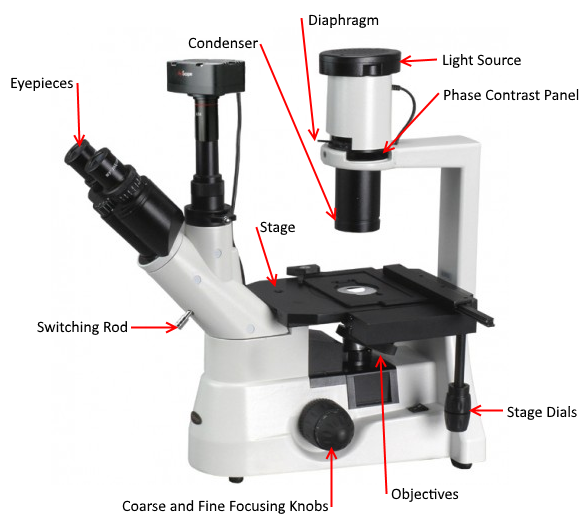
\includegraphics[scale=0.7]{microscope.png}
	\caption{Diagram of the microscope parts.}
	\label{fig:microscope}
\end{figure}

\begin{itemize}
\setlength\itemsep{1pt}
\item Eyepieces
\begin{itemize}
	\setlength\itemsep{1pt}
	\item Adjustable to fit both eyes. If eyelashes obstruct view, move closer to the eyepieces.
%	\item Sometimes easier if one eye is closed
\end{itemize}
\item Light Source, Condenser, Phase Contrast Panel
\begin{itemize}
	\setlength\itemsep{1pt}
	\item Condenser concentrates light from illumination source.
	\item Phase rings in front of the light source allow the microscope to translate phase shifts in light that goes through a transparent sample into brightness changes in the observed images. This allows for very useful imaging of transparent samples that would be difficult with standard bright field imaging.
	\item The light intensity can be controlled by adjusting the orange wheel on the bottom left of the machine.
\end{itemize}
\item Diaphragm
\begin{itemize}
	\setlength\itemsep{1pt}
	\item Lever controls an iris, allowing the user to control the amount of light hitting the sample. Very often, higher detail can be observed by allowing less light through the iris.
\end{itemize}
\item Stage
\begin{itemize}
	\setlength\itemsep{1pt}
	\item Place the sample on the microscope stage carefully. The stage can be moved relative to the objectives using the dials below the stage to the right. Align the sample directly over the objective, so the light is shining directly on the sample.
\end{itemize}
\item Objectives
\begin{itemize}
	\setlength\itemsep{1pt}
	\item Objectives collect the light from the samples and focus it to form an image in the eyepiece or CCD camera. Rotating turret holds four different objective lenses: 4X, 10X, 20X, and 40X. Always start with a low magnification objective: find, center, then focus on the sample before moving on to a higher magnification.
%	\item Always lower objectives using the coarse adjustment knob before rotating the turret.
\end{itemize}
\item Coarse and Fine Focusing Knobs
\begin{itemize}
	\item Bring sample into view using the coarse adjustment knob (inner knob). Once sample is in view, use the fine adjustment knob (outer knob) to achieve the sharpest possible image. Be careful when using the coarse adjustment knob, hitting the slide with the objective can scratch the objective or crack the slide.
\end{itemize}
\item CCD Camera
\begin{itemize}
	\setlength\itemsep{1pt}
	\item Adjust the switching rod to go from eyepiece-only to dual-view mode. Camera can be rotated using the adjustable pin below the lens
\end{itemize}
\end{itemize}

\newpage

\section*{Microscope Software}
The capture software for the microscope is called ``Amscope'', it should be located on the desktop.
The software has a viewing area in the center and adjustment settings on the left.
To begin, click `MU503' under `Camera List' to see the view from the camera in the viewing area.
Then adjust the following settings:
\begin{itemize}
\item Set the `Live' and `Snap' resolutions. While capturing video it's best to use `1280 x 960'.
\item Uncheck `Auto Exposure'. Adjust the `Exposure Time' to approximately 33 ms, this means you will be capturing video at 30 fps. Turn the Gain down to 1.0, increase this if you cannot get a bright enough image.
\item In `Color Adjustment', reduce Saturation to 0 and Contrast to 100. Adjust the brightness as necessary.
\end{itemize}
\paragraph*{To capture a video:}
See figure \ref{fig:am-cap} while following along with the steps below:
\begin{itemize}
\item Click the `Record' button on the left, this will open a window called `Video file'.
\item Type the name of the video file that you want to capture; select your group's data folder as the save location. Click Next
\item select the `avi' format, click Next.
\item Under `Encoder' setect `None Compressor', leave the encode parameter quality set at 100. Click Next.
\item Check the box next to `Time Limit', then input the number of seconds that you want to capture video. Clicking `Finish' (or pressing Enter) will begin the video capture.
\end{itemize}
The microscope can be very sensitive to table vibrations, especially when you are imaging at high magnifications. 
After setting all the video capture parameters, wait a bit before starting the capture for the vibrations to die down.
While the camera is capturing, do your best to not disturb the table.

\paragraph*{To capture a `low fps' video:}
Occasionally we may need to capture video at a low frame rate over a long period of time.
To do this, we will set the software to capture an image every few seconds (see figure \ref{fig:low-fps}).
Then, we will use ImageJ to stitch the images together into a .avi video.
\begin{itemize}
\item Navigate to `Capture $>$ Start Time-lapse (Auto Capture)...'
\item In the window that opens, begin by setting the directory where you want all the images to be saved. It's advised that you create a new folder where you will save all the images, as this will make the rest of the steps easier.
\item Under File, set `Name Format' to `nnnn (sequence)', in `File Prefix' input the names that you want given to the videos, set `File Type' to png.
\item Under Capture Mode, select `Time Slot' and input the number of seconds between each frame.
\item Check `Total Images', then input the number of frames that you want captured.
\item Clicking OK or pressing Enter will begin the time-lapse. As before, wait for the vibrations to die down before beginning the capture, and avoid touching the table.
\item After the time-lapse is complete, open ImageJ and navigate to `File $>$ Import $>$ Image Sequence...'.
\item Navigate to the folder where your time-lapse images are saved, choose any of the images and click Open.
\item In the Sequence Options window, make sure `Sort names numerically' is checked, then click OK.
\item After processing the images, a new window will open. Navigate to `File $>$ Save As $>$ AVI...'. Set Compression to `Uncompressed', set Frame Rate to 25, click OK. Enter the file name, then press Save.
\item After creating the avi file, delete the time-lapse images to avoid using unnecessary space.
\end{itemize}

\begin{figure}[ht]
	\centering
	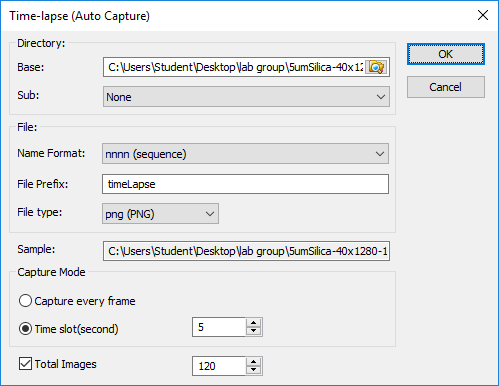
\includegraphics[width=0.7\textwidth]{amscope06}
	\caption{Amscope `low fps' video capturing settings.}
	\label{fig:low-fps}
\end{figure}

\begin{figure}[ht]
	\centering
	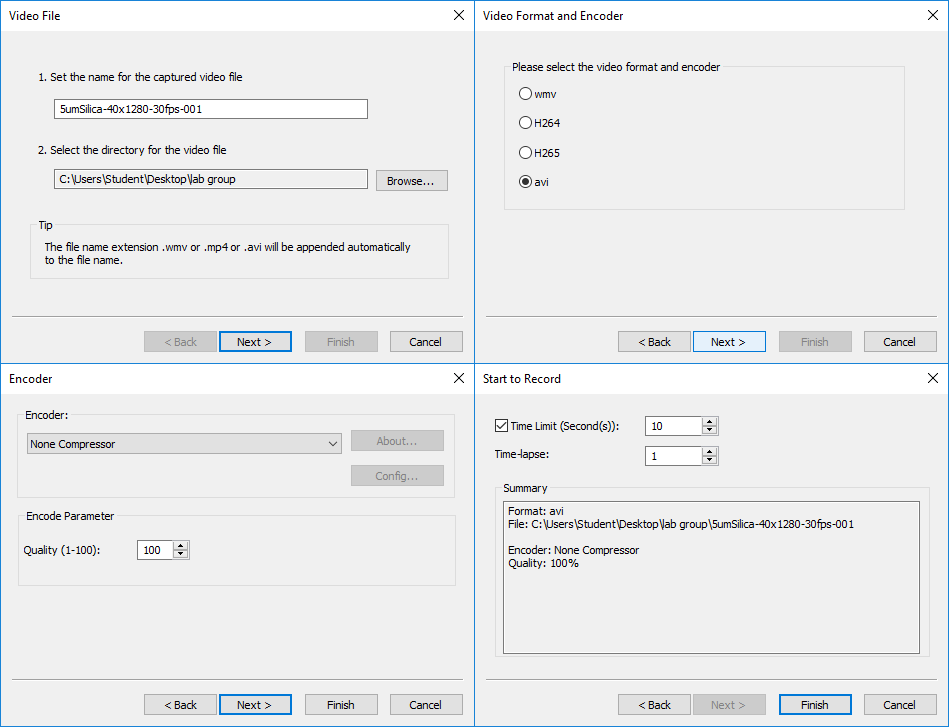
\includegraphics[width=\textwidth]{amscope08}
	\caption{Amscope video capturing settings.}
	\label{fig:am-cap}
\end{figure}


%\section*{Eyepieces:}
%\begin{itemize}
%	\setlength\itemsep{1pt}
%	\item Adjustable to fit both eyes
%	\item Sometimes easier if one eye is closed
%	\item If eyelashes obstruct view, move closer to the eyepieces
%\end{itemize}
%
%\section*{Light Source, Condenser, Phase Contrast Panel:}
%\begin{itemize}
%	\setlength\itemsep{1pt}
%	\item Condenser concentrates light from illumination source
%	\item Phase rings in front of the light source allow the microscope to translate phase shifts in light that goes through a transparent sample into brightness changes in the observed images. This allows for very useful imaging of transparent samples that would be difficult with standard bright field imaging.
%	\item The light intensity can be controlled by adjusting the orange wheel on the bottom left of the machine.
%\end{itemize}
%
%\section*{Diaphragm:}
%\begin{itemize}
%	\setlength\itemsep{1pt}
%	\item Lever controls an iris, allowing the user to control the amount of light hitting the sample
%	\item Very often, higher detail can be observed by allowing less light through the iris
%\end{itemize}
%
%\section*{Stage:}
%\begin{itemize}
%	\setlength\itemsep{1pt}
%	\item Place the sample slide on the microscope stage carefully
%	\item The stage can be moved relative to the objectives using the dials below the stage to the right
%	\item Align the sample directly over the objective, so the light is shining directly on the sample
%\end{itemize}
%
%\section*{Objectives:}
%\begin{itemize}
%	\setlength\itemsep{1pt}
%	\item Objectives collect the light from the samples and focus it to form an image in the eyepiece or CCD camera.
%	\item Rotating turret holds four different objective lenses: 4X, 10X, 20X, and 40X
%	\item Always start with a low magnification objective: find, center and focus on the sample before moving on to a higher magnification.
%	\item Always lower objectives using the coarse adjustment knob before rotating the turret
%\end{itemize}
%
%\section*{Coarse and Fine Focusing Knobs:}
%\begin{itemize}
%	\setlength\itemsep{1pt}
%	\item Bring sample into view using the coarse adjustment knob (inner knob)
%	\item Once sample is in view, use the fine adjustment knob (outer knob) to achieve the sharpest possible image.
%	\item Be careful when using the coarse adjustment knob, hitting the slide with the objective can scratch the objective or crack the slide.
%\end{itemize}
%
%\section*{CCD Camera:}
%\begin{itemize}
%	\setlength\itemsep{1pt}	
%	\item Camera can be rotated using the adjustable pin below the lens
%\end{itemize}		%G
\newpage{\blankpage}
\chapter{Log-Log Plots}
\thispagestyle{fancy}
\fancyhead[RE,LO]{Technical Document \thechapter}
\label{chap:log-plots}

In understanding how one variable depends on another, we introduced the idea of \emph{functional dependence}.
This helps us understand not just that one variable depends on another, but how it depends on the other.
This is especially important in complex situations such as biology where many variables can be involved and "which one dominates" matters.

\section{Powers \& Exponents}

\subsection*{Powers}
Some of the most useful and convenient functional dependencies that we will encounter are \textbf{power laws}.
This means that the variable we choose to be `dependent' depends on the variable we choose to be `independent' by some power of that variable.
Thus
\[ y = f(x) = x^{N} = x \text{ multiplied by itself } N \text{ times} \]
says that ``\emph{y goes like x raised to the Nth power}''.
Note that a power law is not referred to as an ``exponential dependence'' even though the variable ``has an exponent''.
That terminology is reserved for the case when the variable is in the exponent.

\subsection*{Exponentials}
We know that a quadratic function rises faster than a linear one (eventually) and a cubic rises faster than a quadratic.
But there is an extremely useful function that eventually rises faster than any power.
This is the exponential function.
In this case, the variable is not raised to a power - the variable itself is in the power that some constant is raised to.
So as the variable gets bigger and bigger, the power the constant is raised to gets bigger and bigger.
\par
We write
\[ y = e^{x} \text{.} \]
Now e could be any constant, but we typically take it as a special transcendental number (that means it's decimal representation never stops and never repeats): $e = 2.712...$

\subsection*{Logarithms}
The exponential function does the interesting thing of converting sums into products.
If $R = e^{a}$ and $S = e^{b}$ then $R \cdot S = e^{a+b}$.
So if $f(x) = e^{x}$ then we have
\[ f(x_{1})f(x_{2}) = f(x_{1} + x_{2}). \]
Since multiplying is harder than adding, it's sometimes useful to go backwards from the exponential function. 
Taking the exponential of $x$ and setting $y = e^{x}$, if we are given $x$ we can use our calculator (or series) to find $y$.
But what if we are given $y$ and want to find $x$?
The answer to that is called the \emph{natural logarithm} of $y$.
So that would give us the equation:
\[ x = ln(y) \]
Plugging this equation back into our original equation gives:
\[ y = e^{ln(y)} \]
This shows that the natural log ($ln$) is the \emph{inverse function} of the exponential.
If we first take the natural log and then exponentiate it, we get back what we started with.
It works the other way too:
\[ x = ln(e^{x}) \]
If we exponentiate first and then take the natural log, we get back what we started with.
So the natural log function ($ln$) undoes the exponential function and vice versa.
We will see in the following sections that logarithms and exponentials are very useful in analyzing data and seeing whether something behaves like a power law. 

\section{Log-Log Plots}
Power law equations are often used in science to approximate more complicated functions.
%When we have a complicated function it is sometimes useful to approximate it by a simple power law.
However, when these types of equations are plotted on a standard linear graph it can be difficult to recognize the differences between two functions with similar (but not equal) powers.
What we need to do is perform an easily-invertible operation on all our data that also emphasizes changes in power laws. 
One way to see how to do this is to use a \emph{log-log plot}.
Instead of just plotting the variables themselves, we plot the logarithm of the variables.
Let's see how this works.
\par
Suppose we have a power law function $y = ax^{N}$.
If we plot this, we get curves like those in the left side of figure~\ref{fig:lin-log}.
The higher the power we have, the faster it rises (and the odd powers are negative for negative values of x.)
But if we take the logarithm of both sides of that equation, $y = ax^{N}$,we get
\[ log(y)=N \cdot log(x) + log(a) \] 
If we now take as new variables $Y = log(y)$, $X = log(x)$, and $b = log(a)$ then our new equation is just
\[ Y = N \cdot X + b \]
This is the graph of a straight line and the slope is proportional to the power.
If we plot this we get the graph at the right in figure~\ref{fig:lin-log}.

\begin{figure}[ht]
	\centering
	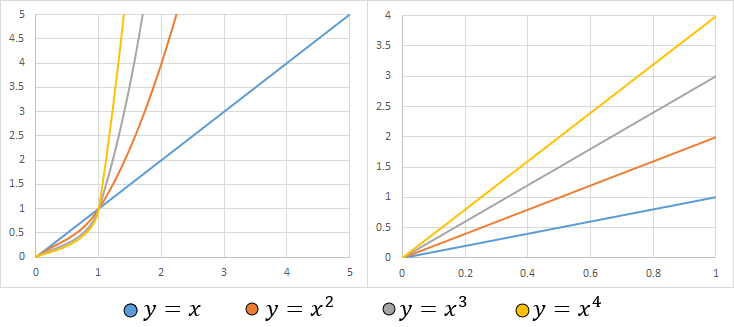
\includegraphics[width=0.8\linewidth]{linVSlog.png}
	\caption{Comparison of linear vs. log-log graphs.}
	\label{fig:lin-log}
\end{figure}

\newpage

All the power laws are straight lines with increasing slope as the powers go up.
So if we are interested in determining if some complicated function can be approximated by a power law, we can easily see if this is the case by plotting the logarithms of the variables. 
If we get a straight line, a power law works. 
(We have only plotted positive values of x and y in the log-log plot since the log of a negative number is not a real number.
Note that this works for negative powers too.) 

%\section{Log-Log Plots in Science}
%Log-Log plots have many uses in science.
%They are especially helpful for differentiating between different forms of \emph{functional dependency}.
%What is functional dependency? 
%Functional dependency tells us how one quantity varies when another is adjusted. 
%Example: for purely random motion, the diffusion of an object in 2-D space has a functional dependence like $\langle r^{2} \rangle = 4 D \Delta t$. 
%As you saw in lab, the viscosity and temperature of the fluid medium surrounding the object and the size of the object can affect the value of the diffusion constant, D, and thus the linear slope of the $\langle r^{2} \rangle$ vs.\ $\Delta t$ plot (where the slope is related to D). 
%A $log(\langle r^{2} \rangle)$ vs.\ $log(\Delta t)$ plot of this functional dependency would be a line with a slope of 1 — regardless of the value of the diffusion constant, D! 
%If we are not learning the diffusion constant D from this log-log plot, what does the slope of 1 tell us?
%\par 
%It turns out that the slope of $log(\langle r^{2} \rangle)$ vs.\ $log(\Delta t)$ tells us about what type of motion we are observing! 
%Most motion will not be linear in an $\langle r^{2} \rangle$ vs.\ $\Delta t$ plot. 
%There are other functional dependencies that can exist governing the relationship between $\langle r^{2} \rangle$ and $\Delta t$. 
%For directed motion at constant velocity, $\langle r^{2} \rangle$ changes as $(\Delta t)^{2}$ and so the $\langle r^{2} \rangle$ vs.\ $\Delta t$ plot would be quadratic. 
%But a $log(\langle r^{2} \rangle)$ vs.\ $log(\Delta t)$ plot of this motion is still linear, with a slope of 2. 
%For directed motion under uniform acceleration from rest, the distance traveled is $r = \frac{1}{2} a \Delta t^{2}$, so $\langle r^{2} \rangle$ changes linearly with $(\Delta t)^{4}$ — thus a $log(\langle r^{2} \rangle)$ vs.\ $log(\Delta t)$ plot of this motion has a slope of 4!
%\par 
%Other motion in cells is confined, e.g. molecules that are caged by a surrounding scaffolding of actin, or molecules on the membrane that are confined to a ``lipid raft'' or patch of membrane that has some functional activity. 
%For such caged motion, $\langle r^{2} \rangle$ does not quite increase linearly with $\Delta t$ — the distance moved gets smaller than we would expect for random motion as we get to larger and larger distances — thus a $log(\langle r^{2} \rangle)$ vs.\ $log(\Delta t)$ plot of this motion has a slope of less than 1.
% \par
%For real biological systems, the motion is often a combination of random and directed motion — and thus a $log(\langle r^{2} \rangle)$ vs.\ $log(\Delta t)$ plot of this motion has a slope between 1 and 2. 
%The dominant functional dependency (the one that determines the type of motion we observe) can also depend on the time scale at which we observe the motion.
%\par
%This is all very interesting, but how is it helpful to us?
%In biology, almost all motion can look quite random, but that apparently random motion can hide other processes that may look similar to random motion — in particular, caged motion:
%
%\begin{figure}[h!]
%	\centering
%	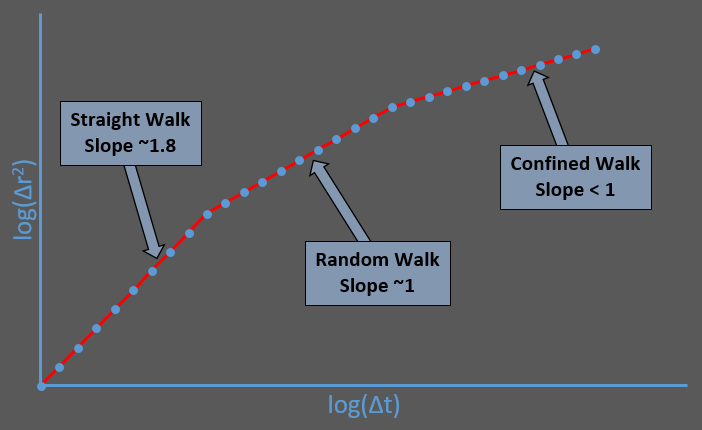
\includegraphics[width=0.6\linewidth]{log_diff.png}
%	\caption{Example investigation of live motion analysis using log-log plots.}
%	\label{fig:log-diff}
%\end{figure}
%
%\begin{itemize}
%\item In ecology, tracking data from tagged animals can be analyzed to find the roaming grounds of an animal.
%However, to distinguish random motion from the confined area to which an animal intentionally returns, we cannot simply look at the tracks by eye.
%A log-log plot can help us find the distances at which the motion gets confined; helping us determine the size of roaming grounds and how often roaming grounds are changed.
%In addition, on shorter timescales the motion will look directed since animals are able to move straight (at least over short distances)!
%\item On much smaller scales, within cells, the tracking data from individual molecules on a cell membrane have helped develop the theory of ``lipid rafts''. Such rafts are patches of membrane that float on the overall cell membrane. Within the raft sit a number of functional molecules that appear to operate together, taking advantage of their closeness to each other within a raft to enhance signals. The significance of lipid rafts in biology is still under investigation and log-log plots are a key tool to distinguish randomness from caged motion!
%\end{itemize}
%
%This particular choice is because when we make this choice, the function ex is its own derivative.
%That is, if we write $y = e^{x}$, then
%\[ \frac{dy}{dx} = y \text{.} \]
%\par
%In case you wondered how in the world a calculator figures out what ``$e$'' to the something is, the following result allows you to calculate the value of $e$ raised to some number -- eventually.
%\[ e^{x} = 1 + x + \frac{x^{2}}{2} + \frac{x^{3}}{6} + \frac{x^{4}}{24}+... \]
%You can see how this goes on - and it goes on forever.
%But for any fixed $x$ you are calculating for, the denominators go up faster than powers do, making the terms smaller and smaller so they can be dropped.
%\par 
%While this looks really messy and we're not going to use it, looking at it does give us two interesting messages.
%\begin{enumerate}
%\item \textbf{It explains why the exponential function is its own derivative.} If you take the derivative of the power series representation of the exponential, something interesting happens. The first term vanishes, the derivative of the linear term becomes the old first term (1), the derivative of the third (quadratic) term becomes the old second (linear) term, etc.  So the derivative of each term becomes the previous term in the original series.  We wind up getting the same thing back that we started with.  This also shows us why the denominators have the structure they do. [And with a little fancy mathematical footwork, we can show that the exponential is the only function that is its own derivative.]
%\item \textbf{It shows that we can only take exponentials of pure numbers.} Since we know that you can't add a length and an area - or any quantity that has units to its square - the power series only makes sense if ``x''  is a pure number.  You can't take an exponential of a quantity that has units.  Whenever in science we have an exponential, it will always be the ratio of two quantities with the same units - typically a variable and a scale for that variable.  (Like a time and a rate constant.)
%\end{enumerate}
%
%\section{Log-log Plots in Science}
%Log-Log plots have many uses in science.
%They are especially helpful for differentiating between different forms of \emph{functional dependency}.
%What is functional dependency? 
%Functional dependency tells us how one quantity varies when another is adjusted. 
%Example: for purely random motion, the diffusion of an object in 2-D space has a functional dependence like $\langle r^{2} \rangle = 4 D \Delta t$. 
%As you saw in lab, the viscosity and temperature of the fluid medium surrounding the object and the size of the object can affect the value of the diffusion constant, D, and thus the linear slope of the $\langle r^{2} \rangle$ vs.\ $\Delta t$ plot (where the slope is related to D). 
%A $log(\langle r^{2} \rangle)$ vs.\ $log(\Delta t)$ plot of this functional dependency would be a line with a slope of 1 — regardless of the value of the diffusion constant, D! 
%If we are not learning the diffusion constant D from this log-log plot, what does the slope of 1 tell us?
%\par 
%It turns out that the slope of $log(\langle r^{2} \rangle)$ vs.\ $log(\Delta t)$ tells us about what type of motion we are observing! 
%Most motion will not be linear in an $\langle r^{2} \rangle$ vs.\ $\Delta t$ plot. 
%There are other functional dependencies that can exist governing the relationship between $\langle r^{2} \rangle$ and $\Delta t$. 
%For directed motion at constant velocity, $\langle r^{2} \rangle$ changes as $(\Delta t)^{2}$ and so the $\langle r^{2} \rangle$ vs.\ $\Delta t$ plot would be quadratic. 
%But a $log(\langle r^{2} \rangle)$ vs.\ $log(\Delta t)$ plot of this motion is still linear, with a slope of 2. 
%For directed motion under uniform acceleration from rest, the distance traveled is $r = \frac{1}{2} a \Delta t^{2}$, so $\langle r^{2} \rangle$ changes linearly with $(\Delta t)^{4}$ — thus a $log(\langle r^{2} \rangle)$ vs.\ $log(\Delta t)$ plot of this motion has a slope of 4!
%\par 
%Other motion in cells is confined, e.g. molecules that are caged by a surrounding scaffolding of actin, or molecules on the membrane that are confined to a ``lipid raft'' or patch of membrane that has some functional activity. 
%For such caged motion, $\langle r^{2} \rangle$ does not quite increase linearly with $\Delta t$ — the distance moved gets smaller than we would expect for random motion as we get to larger and larger distances — thus a $log(\langle r^{2} \rangle)$ vs.\ $log(\Delta t)$ plot of this motion has a slope of less than 1.
% \par
%For real biological systems, the motion is often a combination of random and directed motion — and thus a $log(\langle r^{2} \rangle)$ vs.\ $log(\Delta t)$ plot of this motion has a slope between 1 and 2. 
%The dominant functional dependency (the one that determines the type of motion we observe) can also depend on the time scale at which we observe the motion.
%\par
%This is all very interesting, but how is it helpful to us?
%In biology, almost all motion can look quite random, but that apparently random motion can hide other processes that may look similar to random motion — in particular, caged motion:
%\begin{itemize}
%\item In ecology, tracking data from tagged animals can be analyzed to find the roaming grounds of an animal.
%However, to distinguish random motion from the confined area to which an animal intentionally returns, we cannot simply look at the tracks by eye.
%A log-log plot can help us find the distances at which the motion gets confined; helping us determine the size of roaming grounds and how often roaming grounds are changed.
%In addition, on shorter timescales the motion will look directed since animals are able to move straight (at least over short distances)!
%\item On much smaller scales, within cells, the tracking data from individual molecules on a cell membrane have helped develop the theory of ``lipid rafts''. Such rafts are patches of membrane that float on the overall cell membrane. Within the raft sit a number of functional molecules that appear to operate together, taking advantage of their closeness to each other within a raft to enhance signals. The significance of lipid rafts in biology is still under investigation and log-log plots are a key tool to distinguish randomness from caged motion!
%\end{itemize}
%%
%Below is a chart to help summarize the broad categories of functional dependency and their effects on the slope of the $log(\langle r^{2} \rangle)$ vs.\ $log(\Delta t)$ plots.
%
%
%\begin{table}[h!]
%	\centering
%	\begin{tabular}{|l|c|}
%	\hline 
%	Type of motion & Slope of the $log(\langle r^{2} \rangle)$ vs.\ $log(\Delta t)$ plot \\ 
%	\hline 
%	Confined & $s < 1$ \\ 
%	\hline 
%	Random & $s = 1$ \\ 
%	\hline 
%	Biological & $1 < s < 2$ \\ 
%	\hline 
%	Directed & $s = 2$ \\ 
%	\hline 
%	Accelerated & $s > 2$ \\ 
%	\hline 
%	\end{tabular} 
%	\caption{The effect of movement type on a log-log plot.}
%	\label{tab:logPlt}
%\end{table}
%These types of plots can also help us model a new phenomenon. 
%Imagine a situation in which you wish to develop a model of how a biological or chemical process spreads in space with increasing time. 
%Knowing the functional dependency between $\langle r^{2} \rangle$ and $\Delta t$ can help you build a model or help you choose between competing models. 
%Once we understand the model better, we can make predictions about what will happen when we make changes to the system. 
%In order to help us with our modeling, we take data on the motion and make a plot of $log(\langle r^{2} \rangle)$ vs.\ $log(\Delta t)$. 
%The slope of this plot helps us make decisions about what models to propose or what models to eliminate. 
%It also tells us which functional dependency dominates at which time scales — it tells us when a type of motion is the most important and when we can ignore the effects of other types of motion.
%\par
%(Note that log-log plots help with functional dependencies more generally. 
%In chemistry, you may need to plot the log of a molecule's solubility vs.\ the pH.
%Since the pH is the log of the number of free hydrogen ions, this is again a log-log plot in disguise! 
%Then the slope can tell you how many charges an atom or molecule has in solution.)
			%H

\end{document}